\documentclass{article}

% file's preambule
%%%%%%%%%%%%%%%%%%%



% connect packages
\usepackage[T2A]{fontenc}
\usepackage[utf8]{inputenc}
\usepackage[english]{babel}
\usepackage{hyperref}     % ТАК_НУЖНО
\hypersetup{unicode=true} % ТАК_НУЖНО
\usepackage{amsmath}
\usepackage{amssymb,textcomp, esvect,esint}
\usepackage{amsfonts}
\usepackage{amsthm}
\usepackage{graphicx}
\usepackage{indentfirst}
\usepackage{xcolor}
% \usepackage{enumitem} %--- ломал нумерацию!?

\usepackage{graphicx}
\usepackage{booktabs}
\usepackage{caption}
\usepackage{listings}
\usepackage{tikz}
\usepackage{xcolor}



\usepackage{media9}
\usepackage{animate}
\usepackage{threeparttable}
\usepackage{pifont}


\usepackage{import}
\usepackage{xifthen}
\usepackage{pdfpages}
\usepackage{transparent}

\usepackage[skip=1pt]{caption}

% create environment

\newtheorem{to_thr}{Thr}[section]
\newtheorem{to_suj}[to_thr]{Suj}
\newtheorem{to_lem}[to_thr]{Lem}
\newtheorem{to_com}[to_thr]{Com}
\newtheorem{to_con}[to_thr]{Con}
\theoremstyle{definition}
\newtheorem{to_def}[to_thr]{Def}


\newenvironment{itemize*}
{
    \begin{itemize}
        \setlength{\itemsep}{1pt}
        \setlength{\parskip}{1pt}}
    {\end{itemize}
}

\newenvironment{enumerate*}
{
    \begin{enumerate}
        \setlength{\itemsep}{1pt}
        \setlength{\parskip}{1pt}}
    {\end{enumerate}
}

\newenvironment{description*}
{
    \begin{description}
        \setlength{\itemsep}{1pt}
        \setlength{\parskip}{1pt}}
    {\end{description}
}


\newenvironment{hw1}
{
    \phantom{42}

    \noindent
    \textbf{Домашнее задание:} \hrulefill
    % \vspace{-2mm}
    % \begin{enumerate*}

}
{
    % \end{enumerate*}
    \vspace{2mm}
    \hrule

    \phantom{42}
}


\newenvironment{hw2}
{
    \phantom{42}

    \noindent
    \textbf{Домашнее задание:} \hrulefill
    \vspace{-2mm}
    \begin{enumerate*}

}
{
    \end{enumerate*}
    \hrule

    \phantom{42}
}

% document palette
\definecolor{ugreen}{RGB}{0, 100, 0}
\definecolor{ured}{RGB}{220, 0, 0}
\definecolor{ugray}{RGB}{90, 90, 90}

% \newcommand{\red}[1]{\textcolor{ured}{#1}}
% \newcommand{\green}[1]{\textcolor{ugreen}{#1}}


\definecolor{grey}{HTML}{666666}
\definecolor{linkcolor}{HTML}{0000CC}
\definecolor{urlcolor}{HTML}{006600}
\hypersetup{
    pdfstartview=FitH,  
    linkcolor=linkcolor,
    urlcolor=urlcolor, 
    colorlinks=true,
    citecolor=blue}

% add (renew) commands
% add (renew) commands

\renewcommand{\Im}{\mathop{\mathrm{Im}}\nolimits}
\renewcommand{\Re}{\mathop{\mathrm{Re}}\nolimits}

\renewcommand{\d}{\, d}
\renewcommand{\leq}{\leqslant}
\renewcommand{\geq}{\geqslant}
\renewcommand{\l}{\left}
\renewcommand{\r}{\right}

\newcommand{\vc}[1]{\mbox{\boldmath $#1$}}
\newcommand{\T}{^{\text{T}}}


\newcommand{\diag}{\mathop{\mathrm{diag}}\nolimits}
\newcommand{\cl}{\mathop{\mathrm{cl}}\nolimits}
\newcommand{\grad}{\mathop{\mathrm{grad}}\nolimits}
\renewcommand{\div}{\mathop{\mathrm{div}}\nolimits}
\newcommand{\rot}{\mathop{\mathrm{rot}}\nolimits}
\newcommand{\Ker}{\mathop{\mathrm{Ker}}\nolimits}
\newcommand{\Spec}{\mathop{\mathrm{Spec}}\nolimits}
\newcommand{\sign}{\mathop{\mathrm{sign}}\nolimits}
\newcommand{\tr}{\mathop{\mathrm{tr}}\nolimits}
\newcommand{\rg}{\mathop{\mathrm{rg}}\nolimits}


\newcommand{\DS}{\mathcal D\left(\mathbb{R}\right)}
\newcommand{\QED}{\textnormal{Q. E. D.}}
\newcommand{\dseq}{\overset{\mathcal D'}{=}}
\newcommand{\dto}{\overset{\mathcal D'}{\to}}


\newcommand{\const}{\text{const}}
\newcommand{\xmark}{\ding{55}}


\newenvironment{uproof}{
% \begin{comment}
\par \color{ugray}
\begin{proof}[$\triangle$]
}{
\end{proof} \par
% \end{comment}
}


\newcommand{\bhat}{\overset{\text{\scalebox{0.8}[0.5]{\rotatebox[origin=c]{180}{$\wedge$}}}}}

\newcommand{\cf}[1]{\text{\raisebox{1.5pt}{$\scalebox{1.3}{$\chi$}$}}_{#1}}

\newcommand{\supp}{\mathop{\mathrm{supp}}\nolimits}
\newcommand{\si}{\mathop{\mathrm{Si}}\nolimits}

\newcommand{\rr}{\rightrightarrows}

% \newcommand{\sbsnum}[2]{
%     \setcounter{subsection}{\the\numexpr #1 - 1 \relax}
%     \subsection{#2}
% }

% Секции и сабсекции
% \definecolor{darkblue}{HTML}{000099}
% \newcommand{\sbs}[1]{\subsection{\textcolor{darkblue}{#1}}}
% \renewcommand{\sec}[1]{\section{\textcolor{darkblue}{#1}}}
\newcommand{\sbs}[2]{
\setcounter{subsection}{\numexpr #1 - 1 \relax}
    \textcolor{ugreen}{
        \subsection{#2}
        }
}



% add page header
% add page header

\pagestyle{fancy}
\fancyhf{}
\fancyhead[RE,LO]{\textsc{Ф\raisebox{-1.5pt}{и}з\TeX}}
\fancyhead[LE,RO]{Ж\raisebox{-1.5pt}{и}К}
\fancyhead[CO,CE]{\leftmark}
\fancyfoot[LE,RO]{\textcolor{grey}{\texttt{\thepage}}}



% matrixes shortcuts 
% \newcommand{\dmat}[4]{
  \ifthenelse{
    \equal{#1}{3}
  }{
\begin{pmatrix}
    #2 & 0 & 0 \\
    0 & #3 & 0 \\
    0 & 0 & #4 \\
\end{pmatrix}
  }{
  \ifthenelse{
      \equal{#1}{2}
    }{
  \begin{pmatrix}
      #2 & 0 \\
      0 & #3 \\
  \end{pmatrix}
    }{
      \text{\textcolor{red}{error}}
    }
  }
}

\newcommand{\skmat}[4]{
  \ifthenelse{
    \equal{#1}{3}
  }{
\begin{pmatrix}
    0 & -#4 & #3 \\
    #4 & 0 & -#2 \\
    -#3 & #2 & 0 \\
\end{pmatrix}
  }{
  \ifthenelse{
      \equal{#1}{2}
    }{
  \begin{pmatrix}
      0 & #2 \\
      -#2 & 0 \\
  \end{pmatrix}
    }{
      \text{\textcolor{red}{error}}
    }
  }
}

% additional symbols and commands


\DeclareRobustCommand{\tmpsim}{ %%%%%%%%%%%%%% ~ < %%%%%%%%%%%%%%%%%%%
  \mathbin{\text{
      \raisebox{-1pt}{
            \hspace{-4.5pt} \rotatebox{-26}{\scalebox{0.8}[0.7]{$\sim$}}
        }
  }}
}
\def\lesim{{
    \setbox0\hbox{$\ <\ $}
    \rlap{\hbox to \wd0{\hss$\tmpsim$\hss}}\box0
}}
%%%%%%%%%%%%%%%%%%%%%%%%%%%%%%%%%%%%%%%%%%%%%%%%%%%%%%%%%%%%%%%%%%%%%%


\def\letuscom{%%%%%%%%%%%%%%%%%%%%%% ПУСТЬ %%%%%%%%%%%%%%%%%%%%%%%%%%
\mathord{\setbox0=\hbox{$\exists$}%
     \hbox{\kern 0.125\wd0%
           \vbox to \ht0{%
              \hrule width 0.75\wd0%
              \vfill%
              \hrule width 0.75\wd0}%
           \vrule height \ht0%
           \kern 0.125\wd0}%
   }%
}
\newcommand{\letus}{\raisebox{-1.2pt}{$\letuscom$}}
%%%%%%%%%%%%%%%%%%%%%%%%%%%%%%%%%%%%%%%%%%%%%%%%%%%%%%%%%%%%%%%%%%%%%%


\usepackage{arydshln} %%%%%%%%%%%%%%% ЛИНИИ В МАТРИЧКЕ %%%%%%%%%%%%%%%
\makeatletter
  \renewcommand*\env@matrix[1][*\c@MaxMatrixCols c]{%
    \hskip -\arraycolsep
    \let\@ifnextchar\new@ifnextchar
  \array{#1}}
\makeatother
%%%%%%%%%%%%%%%%%%%%%%%%%%%%%%%%%%%%%%%%%%%%%%%%%%%%%%%%%%%%%%%%%%%%%%


\makeatletter %%%%%%%%%%%%%%% КРУЖОЧЕК %%%%%%%%%%%%%%%%%%%%%%%%%%%%%%%
\newcommand*{\encircled}[1]{\relax\ifmmode\mathpalette
\@encircled@math{#1}\else\@encircled{#1}\fi}
\newcommand*{\@encircled@math}[2]{\@encircled{$\m@th#1#2$}}
\newcommand*{\@encircled}[1]{%
  \tikz[baseline,anchor=base]{\node[draw,circle,outer sep=0pt,
                                        inner sep=.2ex] {#1};}}
\makeatother
%%%%%%%%%%%%%%%%%%%%%%%%%%%%%%%%%%%%%%%%%%%%%%%%%%%%%%%%%%%%%%%%%%%%%%












\begin{document}

\setlength{\abovedisplayskip}{3pt}
\setlength{\abovedisplayshortskip}{3pt}
\setlength{\belowdisplayskip}{3pt}
\setlength{\belowdisplayshortskip}{3pt}

% \numberwithin{equation}{section}

\begin{center}
    \LARGE \textsc{Задание по курсу <<Дифференциальные уравнения II>>}
\end{center}

\hrule

\phantom{42}

\begin{flushright}
    \begin{tabular}{rr}
    % written by:
        \textbf{Автор}: 
        & Шишкин П.Е. \\
        &\\
    % date:
        \textbf{От}: &
        \textit{\today}\\
    \end{tabular}
\end{flushright}

\thispagestyle{empty}
\tableofcontents
\newpage



\section{Задача Коши}
\subsection{C. \S5: 26}

а) Нет 
\begin{proof} Предположим существуют 2 различные интегральные кривые g(x), h(x) которые касаются в точке ($x_0$,$y_0$). Тогда:
\begin{equation}
g(x_0)=h(x_0)=y_0
\end{equation}
\begin{equation}
g'(x_0)=h'(x_0)=y_0  
\end{equation}

Рассмотрим Задачу Коши:
\begin{equation}
f(y',y,x)=0
\end{equation}
По теореме о существовании и единственности решения ЗК у данного уравнения существует ровно одно решение с начальным условием $y(x_0)=y_0$ Это означает что h(x) и g(x) совпадает, что противоречит условии о различности. 
\end{proof}
б) Нет. Даказательство полностью аналогично, кроме использования второго начального условия.  
\begin{proof} Предположим существуют 2 различные интегральные кривые g(x), h(x) которые касаются в точке ($x_0$,$y_0$). Тогда:
\begin{equation}
g(x_0)=h(x_0)=y_0
\end{equation}
\begin{equation}
g'(x_0)=h'(x_0)=y_0  
\end{equation}

Рассмотрим Задачу Коши:
\begin{equation}
f(y'',y',y,x)=0
\end{equation}
По теореме о существовании и единственности решения ЗК у данного уравнения существует ровно одно решение с начальными условиями $y(0)=y_0$ $y'(0)=y'_0$Это означает что h(x) и g(x) совпадает, что противоречит условии о различности. 
\end{proof}
в) Да
\begin{proof}
Опять-таки воспользуемся теоремой о существовании и единственности, но здесь нам уже понадобится условие существования а не единственности.
Рассмотрим Задачу Коши:
\begin{equation}
f(y''',y'',y',y,x)=0 
\end{equation}
с начальными условиями $y(0)=y_0$, $y'(0)=y'_0$. Тогда существуют различные решения для $y''(0)=1$ и $y''(0)=963467876436543897658635321$. 
\end{proof}
\subsection{С. \S5: 28a }
Сравним производные $y_1$ и $y_2$. Они пересекаются в точке (0,0) Необходимым условием на n будет:
$$
y_1(0)^{(n-1)} \neq y_2(0)^{(n-1)}
$$
Посчитаем производные \\
$y_1(0)'=1$ $y_1(0)''=0$\\  
$y_2(0)'=1$ $y_2(0)''=2$\\
Таким образом минимальное n будет 2+1=3. Покажем, что этого достаточно:
\begin{proof}
Рассмотрим задачу Коши:
\begin{equation}
y'''=0
\end{equation}
С начальными условиями $y(0)=0$, $y'(0)=1$, $y''(0)=0$ и $y(0)=0$, $y'(0)=1$, $y''(0)=2$. Т.к. решение задачи Коши единственно, этими решениями и будут $y_1$ $y_2$ из условия.
\end{proof}
\subsection{С. \S6: 36 } 
В уравнении 
\begin{equation}
    2 x y^2 y'^2 - y^3 y' + 1 = 0
\end{equation}
Сделаем замену $\frac{d x}{d y}=p$
\begin{equation}
\begin{cases}
    \frac{2 x y^2 }{p^2} - \frac{y^3}{p} + 1 = 0\\
    \frac{d x}{d y}=p
\end{cases}
\end{equation}
Разрешим первое уравнение относительно x 
\begin{equation} \label{sorry_Konstantin}
\begin{cases}
    2 x =p y - \frac{p^2 }{y^2} \\
    \frac{d x}{d y}=p
\end{cases}
\end{equation}
Второе уравнение системы \ref{sorry_Konstantin} можем записать как $dx = p dy$, от первого возьмём дифференциал.
\begin{equation}
\begin{cases}
    (y^3-2p)(y d p - p d y)=0 \\
    \frac{d x}{d y}=p
\end{cases}
\end{equation}
Откуда:
\begin{equation}
\begin{cases}
\left[
\begin{gathered}
    \frac{y^3}{2}=p\\
    \frac{d y}{y} = \frac{d p}{p} \\
\end{gathered}
\right. \\
    2 x =p y - \frac{p^2 }{y^2} \\
\end{cases}
\end{equation}
проинтегрируем второе выражение в совокупности (получим $p=C y$) и подставим оба уравнения совокупности в уравнение на x:
\begin{equation}
    \begin{cases}
    \left[
    \begin{gathered}
        8x=y^4\\
        2x=C y^2 - C^2 \\
    \end{gathered}\right. \\
        2 x =p y - \frac{p^2 }{y^2} \\
    \end{cases}
\end{equation}
Построим графики полученных кривых Рис. \ref{fig:6.36}
\begin{figure}[ht]
\center{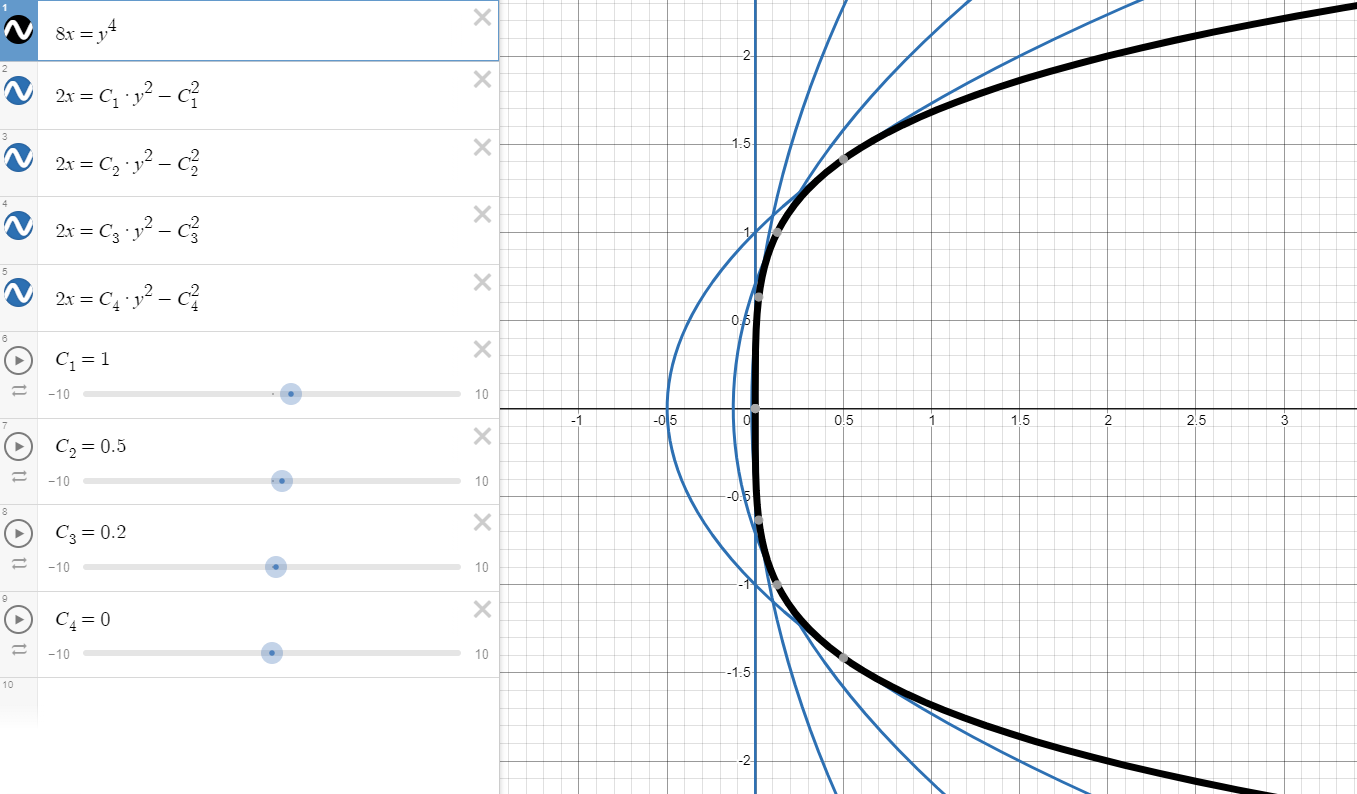
\includegraphics[width=1\linewidth]{6.36.png}}
\caption{Интегральные кривые С. \S6: 36}
\label{fig:6.36}
\end{figure}
\newline
Весьма очевидно, что особым решением, дискриминантной кривой в данном случае будет $8x=y^4$ но, к сожалению, это необходимо доказать :(
\begin{proof}
Необходимое условие дискриминантной кривой:
\begin{equation}
    \begin{cases}
    \frac{\partial}{\partial p}(2 x y^2/p^2 - y^3 /p + 1) = 0\\
    2 x y^2/ p^2 - y^3 /p + 1 = 0\\
    \end{cases}
\end{equation}
Откуда:
\begin{equation}
    \begin{cases}
    p=\frac{y^3}{2}\\
    8x=y^4\\
    \end{cases}
\end{equation}
Как мы видим дискриминантной кривой может быть только $x=y^4/8$, но то что она таковой является надо ещё проверить:
\begin{equation}
    \begin{cases}
    \frac{d}{d y}(\frac{C y^2 - C^2}{2})=\frac{d}{d y}(y^4/8)\\
    \frac{C y^2 - C^2}{2}=y^4/8\\
    \end{cases}
\end{equation}
Что в итоге даёт:
\begin{equation}
    \begin{cases}
    C=\frac{y^2}{2}\\
    0=0
    \end{cases}
\end{equation}
Т.е. $x=y^4/8$ действительно дискриминантная кривая, касающаяся решений  вида $C y^2 - C^2$ при $C \geq 0$
\end{proof}


\subsection{С. \S6: 49 }
Решение полностю аналогично предыдущему, однако в этот раз разрешим уравнение относительно $y$ а не $x$ (это чтобы я не совсем уж весь код копипастил):
В уравнении 
\begin{equation}
    y'-\ln(y')=y-x 
\end{equation}
Сделаем замену $\frac{d y}{d x}=p$ и разрешим первое уравнение относительно $y$ 
\begin{equation}
    \begin{cases}
        y=p - \ln(p) + x\\
        \frac{d y}{d x}=p
    \end{cases}
\end{equation}
Второе уравнение системы (20) можем записать как $dy = p dx$, от первого возьмём дифференциал.
\begin{equation}
    \begin{cases}
        (p-1)(d p - p d x)=0 \\
        \frac{d y}{d x}=p
    \end{cases}
\end{equation}
Откуда:
\begin{equation}
    \begin{cases}
    \left[
    \begin{gathered}
        p=1\\
        \frac{d p}{p} = dx \\
    \end{gathered}
    \right. \\
        y=p - \ln(p) + x \\
    \end{cases}
\end{equation}
проинтегрируем второе выражение в совокупности (получим $p=e^{x+C}$) и подставим оба уравнения совокупности в уравнение на y:
\begin{equation}
\begin{cases}
\left[
\begin{gathered}
    y=1+x\\
    y=e^{x + C} -C \\
\end{gathered} \right. \\
    y=p - \ln(p) + x \\
\end{cases}
\end{equation}
Построим графики полученных кривых Рис. \ref{fig:6.49}
\begin{figure}[ht]
    \center{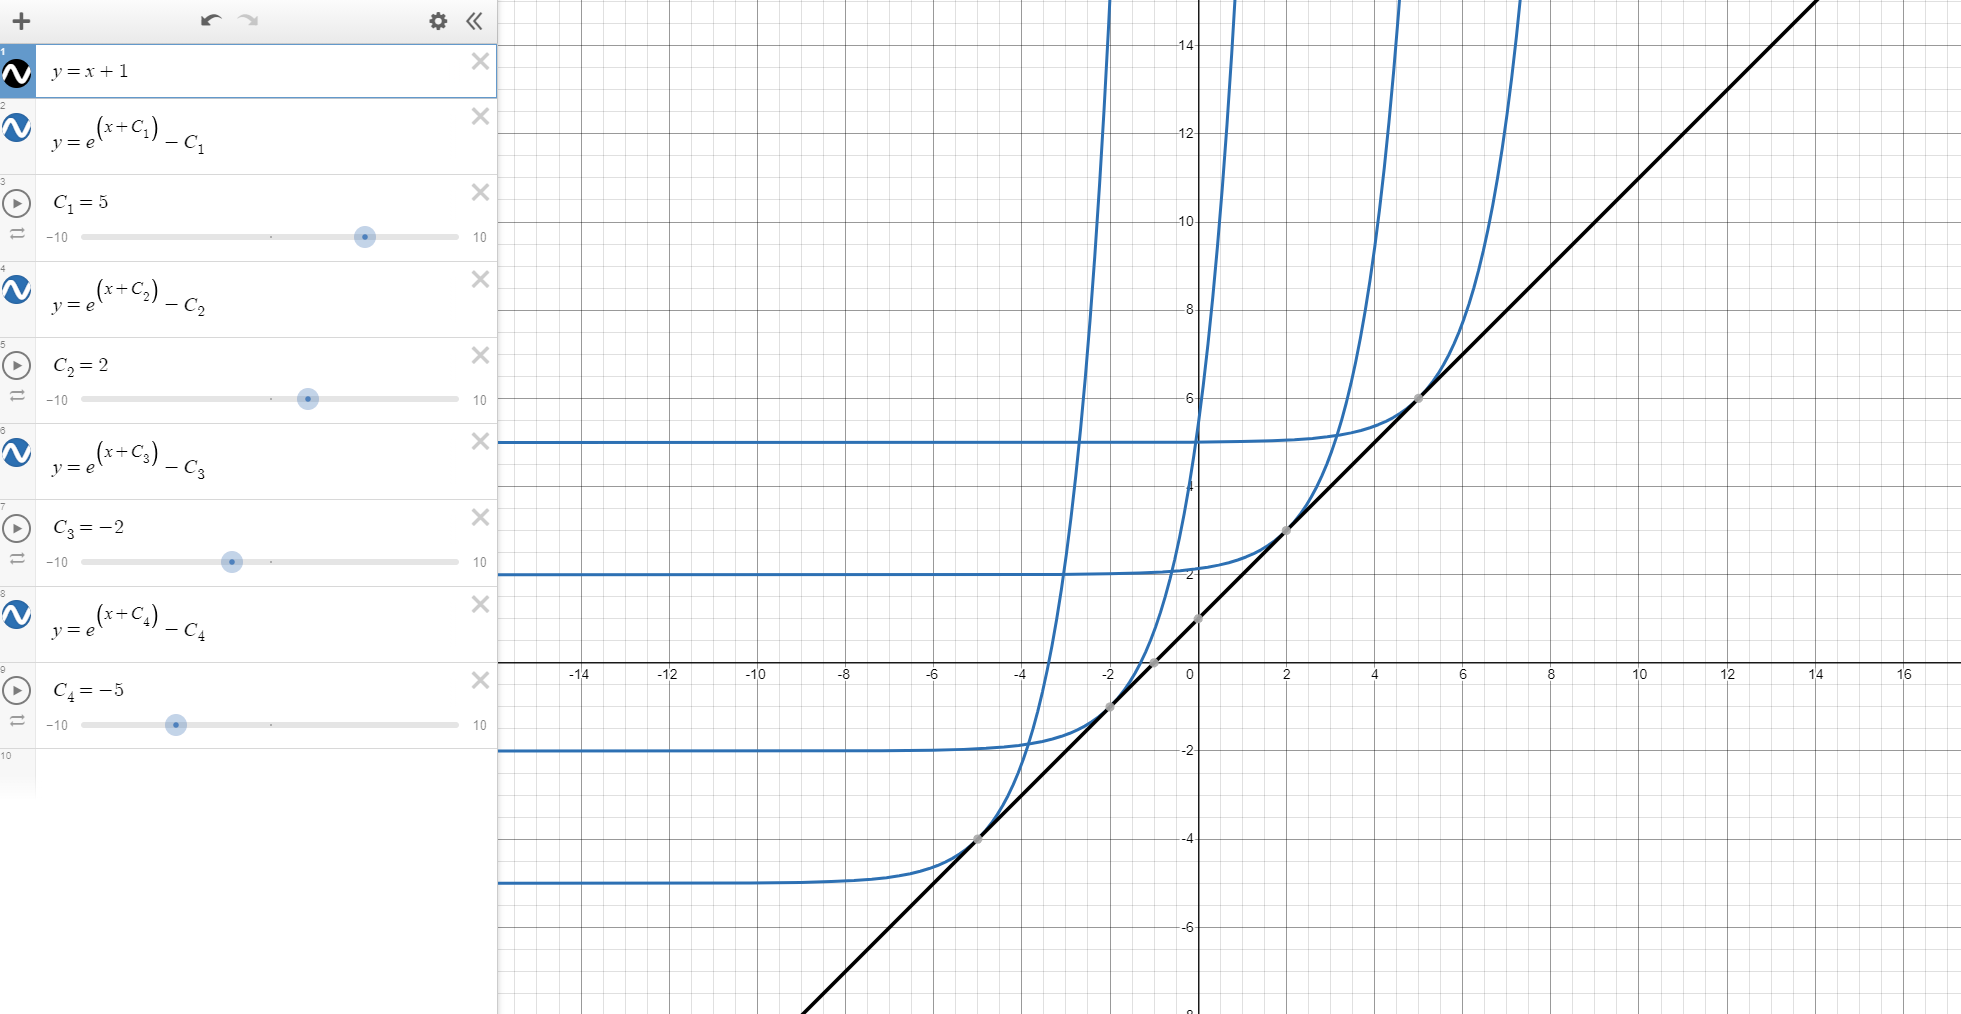
\includegraphics[width=1\linewidth]{6.49.png}}
    \caption{Интегральные кривые С. \S6: 49}
    \label{fig:6.49}
\end{figure}
\newline
Весьма очевидно, что особым решением, дискриминантной кривой в данном случае будет $y=x+1$ но, к сожалению, это необходимо доказать :(
\begin{proof}
Необходимое условие дискриминантной кривой:
\begin{equation}
    \begin{cases}
    \frac{\partial}{\partial p}(p - \ln(p) + x - y) = 0\\
    p - \ln(p) + x -y=0\\
    \end{cases}
\end{equation}
Откуда:
\begin{equation}
    \begin{cases}
    p=1\\
    y=x+1\\
    \end{cases}
\end{equation}
Как мы видим дискриминантной кривой может быть только $y=x+1$, но то что она таковой является надо ещё проверить:
\begin{equation}
    \begin{cases}
    \frac{d}{d x}(e^{x+C}-C)=\frac{d}{d x}(x+1)\\
    e^{x+C}-C=x+1\\
    \end{cases}
\end{equation}
Что в итоге даёт:
\begin{equation}
    \begin{cases}
    x+C=0\\
    0=0
    \end{cases}
\end{equation}
Т.е. $y=x+1$ действительно дискриминантная кривая, касающаяся решений  вида $e^{x+C}-C$ уже (в сравнении с предыдущей задачей) при любых $C$
\end{proof}

\subsection{Ф.: 1065}
Для решения задач 1065-1067 воспользуемся следующим фактом (Филиппов с. 109-110) :\\
Если в системе уравнений 
\begin{equation}
\label{eq2}
    \frac{d x_i}{d t} = f_i(t,x_1, ... , x_n, \mu) 
\end{equation}

с начальными условиями $x_i(0)=a_i(\mu)$ для $i=1,..,n$ \\
$\mu$ является параметром, функции $f_i$ и $a_i$ непрерывны и имеют непрерывные производные по $x_1, ... , x_n, \mu$ , то решение имеет непрерывную производную по параметру $\mu$, а производные $\frac{\partial x_i}{\partial \mu} = u_i$ удовлетворяют линейной системе уравнений \ref{eq1}:
\begin{equation}
\label{eq1}
    \frac{d u_i}{d t} = \sum_{j=1}^n \frac{\partial f_i}{\partial x_j} u_j + \frac{\partial f_i}{\partial \mu}
\end{equation}
и начальным условиям $u_i(0)=a'_i(\mu)$. Значения производных в формуле \ref{eq1} берутся при $x_i=x_i(t)$ - решения системы \ref{eq2} с заданными начальными условиями.\\

Теперь можно порешать задачи:
\begin{equation}
    y'=2x+\mu y^2
\end{equation}
с начальными условиями: $y(0)=\mu-1$. \\
Очевидно решение 
\begin{equation} \label{eq3}
    y(\mu=0)=x^2-1
\end{equation} 
Рассмотрим теперь решение в нуле уравнения \ref{eq1}. Подставим туда очевидное нам решение \ref{eq3} и получим:
\begin{equation} \label{eq4}
    \frac{d u}{d x} = x^4 - 2x^2 +1
\end{equation}
Проинтегрируем \ref{eq4} и получим:
\begin{equation}
    u(x)=x^5/5-2 x^3 /3 + x + C
\end{equation}
Поскольку $u(0)=\frac{d }{d \mu} y(0)=1$ финальным ответом будет:\\
\begin{equation}
    u=x^5/5-2 x^3 /3 + x + 1
\end{equation}
\subsection{Ф.: 1066}
\begin{equation}
    y'= y + y^2 +x y^3
\end{equation}
с начальными условиями: $y(2)=y_0$. \\
Запишем \ref{eq1} для данной задачи:
\begin{equation} \label{eq5}
    \frac{d u}{d x}=(1+2 y + 3x y^2)u
\end{equation}
Подставим в \ref{eq5} начальные условия при которых нас просят найти u: $y=y_0=0$. Проинтегрируем и получим :
\begin{equation}
    u(x)=e^{x+c}
\end{equation}
Осталось только найти константу C. Это тоже не очень трудно: $u(2)=1$ (в качестве $\mu$ мы использовали $y_0$ а значит производная, очевидно, 1). Значит $C = -2$. И конечный ответ:
\begin{equation}
u(x)=e^{x-2}
\end{equation}
\subsection{Ф.: 1067*}
Чтобы скопипастить 1065, ничего не меняя, обозначим $x$ как $y$, $t$  как $x$ 
\begin{equation}
    y'=y/x+\mu x e^{-y}
\end{equation}
с начальными условиями: $y(1)=1$. \\
Очевидно решение 
\begin{equation} \label{eq6}
    y(\mu=0)=x
\end{equation} 
Рассмотрим теперь решение в нуле уравнения \ref{eq1}. Подставим туда очевидное нам решение \ref{eq6} и $\mu=0$ получим:
\begin{equation} \label{eq7}
    \frac{d u}{d x} = u/x + x e^{-x}
\end{equation}
Решим \ref{eq7} и получим:
\begin{equation}
    u(x)= x(C - e^{-x})
\end{equation}
Поскольку $u(1)=0$ (начальные условия от мю не зависят), вернув оригинальные обозначения получим ответ:\\
\begin{equation}
    u(x)= t(e^{-1} - e^{-t})
\end{equation}
\subsection{Т1}
Ну а чего бы ему продолжаться?
\begin{proof}
рассмотрим случай $y>0$ для него решение принимает вид:
\begin{equation}\label{eq8}
    y_1=(\alpha -1)^{\frac{1}{1-\alpha}}(C_1-x)^{\frac{1}{1-\alpha}}
\end{equation}
При $y<0$ решения принимают вид:
\begin{equation}\label{eq9}
    y_1=-(\alpha -1)^{\frac{1}{1-\alpha}}(C_2-x)^{\frac{1}{1-\alpha}}
\end{equation}
 Довольно очевидно, что \ref{eq8} и \ref{eq9} не могут быть продолжены на интервал $(-\infty, + \infty)$ хотя бы из-за того что они не определены на всём интервале. Взять же объединение этих решений невозможно, потому что единственная точка, где они могли бы пересекаться: $y=0$ не достигается ни одним из решений, т.е. объединение решений никогда не будет непрерывной функцией.
\end{proof}

\subsection{T2}
Слишком много пунктов а смысла маловато $\Rightarrow$ плохая задача.\\
Решим квадратное уравнение относительно $y'$, откуда можно получить:
\begin{equation}
    \left[
\begin{gathered}
    y'=1 \\
    y'=y \\
\end{gathered}\\
\right.
\end{equation}
Тогда решениями уравнения будут кривые:
\begin{equation}\label{eq9_}
    \left[
\begin{gathered}
    y_1=x+C_1 \\
    y_2=e^{x+C_2} \\
\end{gathered}\\
\right.
\end{equation}
Покажем, что черезх каждую точку кривой $y=1$ проходит 2 кривые, имеющие общую касательную (производную). Просто приведём пример $C_1(x)$ $C_2(x)$(не следует понимать что $C_1$ и $C_2$ перестали быть константами для кривой, мы лишь смотрим какие константы соответсвуют кривым, проходящим через точку $(x,1)$. 
$e^{x+C_2}=x+C_1=1$ $\Rightarrow $
$\begin{cases} 
C_1=1-x \\ 
C_2=-x
\end{cases}, $
 тогда   $y_1'=y_2'=1$ что соответсвует наличию общей касательной.\\
Решим краевую задачу $y(0)=0, y(2)=e$. Тогда, очевидно из \ref{eq9_} $C_1=0; C_2=-1$. Построим график полученного решения \ref{fig:T2}

\begin{figure}[ht]
\center{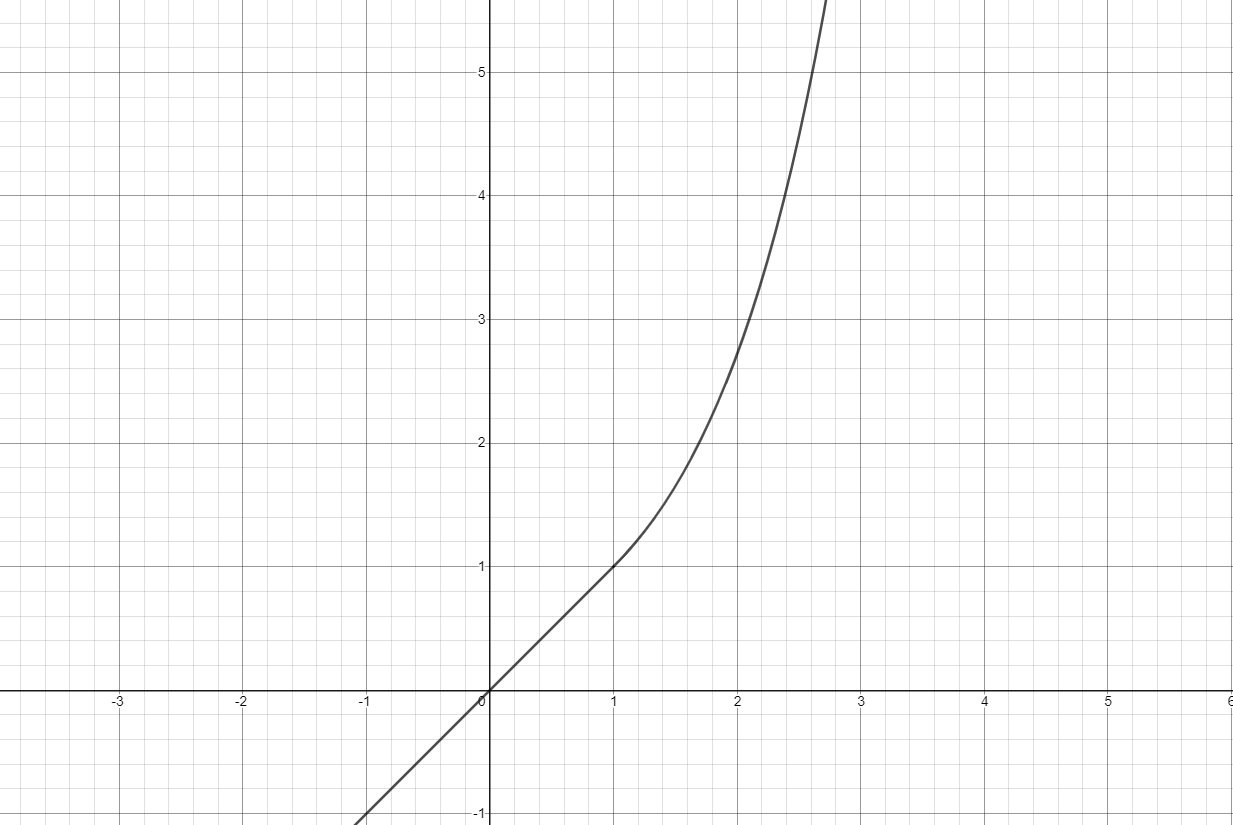
\includegraphics[width=1\linewidth]{T2.png}}
\caption{Решение краевой задачи Т2}
\label{fig:T2}
\end{figure}
\section{Линейные уравнения с переменными коэффициентами}
\subsection{Ф.: 649}
Провероить, являются ли функции $x$, $e^x$, $x e^x$ линейно независимыми на $I=(-\infty,+\infty)$.\\

Метод 1:\\ 
Воспользуемся следующим свойством определителя Вронского: Если функции $f_1(x),...,f_n(x)$ линейно зависимы на $I$, определитель Вронского $W(x)=0$ $\forall x \in I$ (обратное не обязательно верно). Откуда очевидно, что если хотя бы в 1 точке $I$ Вронскиан не 0, то функции линейно независимы (а если W(x) всюду 0, ещё нет гарантии, что функции линейно зависимы, это ещё необходимо проверить).\\
\begin{equation}\label{f649.1}
    W(x) = 
    \begin{vmatrix}
    x && e^x && e^x x \\
    1 && e^x && e^x(x+1)\\
    0 && e^x && e^x(x+2)
    \end{vmatrix}
    =x e^{2x} ((x+2)-(x+1))-1 e^{2x}((x+2)-x) = e^{2x}(x-2)
\end{equation}
Весьма очевидно, выражение \ref{f649.1} $ =0$ не на всём промежутке $I=(-\infty,+\infty)$ (а только в точке $x=2$), а значит есть точка где он не ноль (более того этих точек оч много), что означает что функции линейно независимы.\\

Метод 2: (на самом деле он не нужен для понимания материала, я вообще хз, зачем его написал, но не стирать же):\\
Предположим, фунции линейно зависимы. Тогда:
\begin{equation}\label{f649.2}
    \lambda_1 x + \lambda_2 e^x + \lambda_3 x e^x = 0 \text{ } \forall x \in I
\end{equation}
Поскольку \ref{f649.2} верно для любых $x$ подставим $x=0$,$x=1$,$x=2$, Получим систему:
\begin{equation}
    \underbrace{
    \begin{pmatrix}
    0 && 1 && 0\\
    1 && e && e\\
    2 && e^2 && 2e^2
    \end{pmatrix}}_{A}
    \begin{pmatrix}
    \lambda_1\\
    \lambda_2\\
    \lambda_3
    \end{pmatrix}
    =0
\end{equation}
 Поскольку $det(A)=2 e - 2 e^2 \neq 0$ система имеет только тривиальное решение. Противоречие. 
 \subsection{Ф.: 664}
 Еслич честно, не понимаю смысл задачи. Очевидно, функции линейно независимы, ну докажу что ли...
 \begin{proof}
Предположим функции линейно зависимы, тогда вронскиан тождественно равен нулю на всём промежутке. В то же время в точке $x_1$ $w(x) \neq 0$. Противоречие. Значит функции линейно независимы. 
 \end{proof}

\subsection{Ф.: 667}
Илья Викторович-таки попал в задачу из задания :)
Легко видеть (особенно если решать задачу сразу после семинара где она обсуждалась), что Вронскиан равен нулю. Тем не менее, это ещё не означает, что функции линейно зависимы. Покажем что это не так. Тогда воспользуемся методом 2:
Предположим, фунции линейно зависимы. Тогда:
\begin{equation}\label{f649.2_}
    \lambda_1 x + \lambda_2 x^5 + \lambda_3 |{x^5}| = 0 \text{ } \forall x \in I
\end{equation}
Поскольку \ref{f649.2_} верно для любых $x$, подставим $x=-1/2$,$x=1/4$,$x=1/2$, Получим систему:
\begin{equation}
    \underbrace{
    \begin{pmatrix}
    -1/2 && -1/32 && 1/32\\
    1/4 && 1/1024 && 1/1024\\
    1/2 && 1/32 && 1/32
    \end{pmatrix}}_{\text{ЫуЫа}}
    \begin{pmatrix}
    \lambda_1\\
    \lambda_2\\
    \lambda_3
    \end{pmatrix}
    =0
\end{equation}
 Поскольку $\det(\text{ЫуЫа})=15/32768 \neq 0$ система имеет только тривиальное решение. Противоречие. Значит функции линейно независимы.
 \subsection{Ф.: 668*}
 \begin{proof}

 В данной задаче рассматривается Вронскиан однородного дифф. уравнения 2 порядка. Это весьма важно, т.к. Определитель Вронского однородного дифференциального уравнения либо тождественно равен нулю, и это означает, что $f_{1}(x),\ldots ,f_{n}(x)$ линейно зависимы, либо не обращается в нуль ни в одной точке $I$, что означает линейную независимость функций $ f_{1}(x),\ldots ,f_{n}(x)$. Пусть $g(x)$, $h(x)$ - те самые 2 решения из условия. Тогда:
 \begin{equation}
     W(x)=
     \begin{vmatrix}
      g(x) && p(x) \\
      g'(x) && p'(x)
     \end{vmatrix}
 \end{equation}
Кроме того мы знаем, что в некоторой точке эти функции имеют максимум, т.е. $\exists x_0:$ $g'(x) = p'(x) = 0$ Тогда Вронскиан в $x_0$:
 \begin{equation}
     W(x)=
     \begin{vmatrix}
      g(x_0) && p(x_0) \\
      0 && 0
     \end{vmatrix}
     =0
 \end{equation}
 Что означает линейную зависимость $g(x)$ и $h(x)$.
\end{proof}
Стоит отметить, что если бы функции $g(x)$ и $h(x)$ были не решениями однородного дифф. уравнения 2 порядка, а просто какими-то функциями, то такое доказательство не было бы верно, например: $g(x)=\cos(x)$ $h(x)=-x^2+\pi$ имеют максимум в $(0,0)$, но очевидно линейно независимы.
\subsection{Ф.: 673}
Пристально посмотрим на решения $y_1=x^2-2x+2$, $y_2=x^2-4x+4$, $y_3=x^2+x-1$, $y_4=-x-1$. Можно заметить, что: $y_3+3 y_4=y_1$, $y_3+5 y_4=y_2$. Решения $y_3, y_4$ очевидно линейно независимы. Знгачит есть только 2 линейно независимых решения. Пусть $y(x)$ - общее решение диф уравнения. Оно всегда будет линейно зависимо с частными. Тогда:
\begin{equation}\label{f673.1}
    W(x)=
    \begin{vmatrix}
     y(x)&& y_3 && y_4\\
     y'(x)&& y_3' && y_4'\\
     y''(x)&& y_3'' && y_4''
    \end{vmatrix}
    =0
\end{equation}
Равенство \ref{f673.1} это уже пример д.у. второго порядка. Т.е. $N_{min} \leq 2$. Очевидно, $N_{min} \neq 1$ Потому что у д.у. первого порядка не может быть 2 линейно независимых решений. Откуда получаем ответ: $N\geq 2$
\subsection{Ф.: 678}
Воспользуемся методом из предыдущей задачи: скажем что общее решение д.у. всегда линейно зависимо с наибольшей по включению линейно независимой системой частных решений этого д.у., а значит Вронскиан $W(y(x),f_1,\ldots, f_n)=0$
\begin{align*}
    &y_1(x)=\sh(x), &y_1'(x)=\ch(x), &&y_1(x)''=\sh(x) \\
    &y_2(x)=\ch(x), &y_2'(x)=\sh(x), &&y_2(x)''=\ch(x) 
\end{align*}
$y_3(x)=e^x=y_1(x)+y_2(x)$ это решение не надо писать во Вронскиане, поскольку оно уже линейно зависимо с другими 2\\
Тогда построим д.у.:
\begin{equation}
    W(x)
    =
    \begin{vmatrix}
     y(x) && \sh(x) && \ch(x)\\
     y'(x) && \ch(x) && \sh(x)\\
     y''(x) && \sh(x) && \ch(x)\\
    \end{vmatrix}
    =y''(x) (\sh^2(x)-\ch^2(x)) - y'(x) (\sh(x)\ch(x)-\sh(x)\ch(x)) + y(x) (\ch^2(x)-\sh^2(x))
    =0
\end{equation}
И итоговое д.у. получается весьма красивым: $y''(x)-y(x)=0$
\subsection{Ф. \S22:47*}
Рассмотрим уравнение 
\begin{equation} \label{22:47.1}
(x+2)y''-3y'+y \sqrt{1-x}=0    
\end{equation}
Выражение \ref{22:47.1} запишем в приведённом виде.
\begin{equation}
    y''- \frac{3y'}{(x+2)} + \frac{y \sqrt{1-x}}{x+2}=0 
\end{equation}
а)Т.к. коэффициенты непрерывны только на промежутке $(-2,1]$ то решения можно продолжить не более чем на этот промеждуток. Это оценка сверху. Теперь осталось доказать что решения действительно можно продолжить...
б) в точке 0 детерминант Вронского
\begin{equation*}
W(x=0)=
\begin{vmatrix}
y_1(0) && y_2(0)\\
y_1'(0) && y_2'(0)\\
\end{vmatrix}
=
\begin{vmatrix}
1 && 3\\
0 && 2\\
\end{vmatrix}
= 2 \neq 0
\end{equation*}
Не равен нулю, а значит решения $y_1(x)$ и $y_2(x)$ линейно независимы и составляют фундаментальную систему.
в) Для нахождения $W(x=-1)$ воспользуемся формулой Лиувилля — Остроградского: \\
Пусть есть уравнение вида:
\begin{equation}
    y^{(n)}+P_{1}(x)y^{(n-1)}+P_{2}(x)y^{(n-2)}+...+P_{n}(x)y=0,
\end{equation}
тогда:
\begin{equation}
    W(x)=W(x_0) e^{-\int_{x_0}^x P_1(t)dt}
\end{equation}
Тогда для нашей задачи:
\begin{equation}
    W(x=-1)=W(x_0) e^{-\int_{x_0}^{-1} P_1(t)dt}=2 e^{-\int_{0}^{-1} \frac{-3}{t+2}dt}=2 e^{-\ln(8)}=1/4
\end{equation}
\subsection{Ф. \S22:59}
Обозначим искомое решение как $y_{\text{ЫуЫа}}$
Т.к. известны три частных, можем найти базисные решения, как разность частных:\\
$\varphi_1=y_1-y_2 = x^2+x-1$\\
$\varphi_2=y_2-y_3 = 2x$\\
Таким образом общее решение Д.У. будет иметь вид:
\begin{equation}
    y(x)=C_1\varphi_1+C_2\varphi_2+y_1=C_1(x^2+x-1)+C_2x+x^2
\end{equation}
и, очевидно:
\begin{equation}
    y'(x)=C_1(2x+1)+C_2+2x
\end{equation}
Здесь двойку из решения $\varphi_2$ я внёс под константу, ну потому что лень с ней работать.\\
Подберём теперь константы $C_1$ и $C_2$ для наших начальных условий.
\begin{equation}
    y(0)=2=C_1(0^2+0-1)+0 C_2+0^2=-C_1
\end{equation}
\begin{equation}
    y'(0)=0=C_1(2\cdot 0+1)+C_2+2 \cdot 0=C_1+C_2
\end{equation}
Таким образом: $C_1=-2$ и $C_2=2$, откуда: $y_{\text{ЫуЫа}}=-x^2+2$
\subsection{С. \S9: 10 }
Решить уравнение 
\begin{equation}
    2 x y'' + (4x+1)y' + (2x+1)y=e^{-x}, x>0
\end{equation}
1) угадаем первое решение О.Д.У в виде $\varphi_1(x)=e^{\alpha x}$.
\begin{equation}
    2x e^{\alpha x} \alpha^2 + (4x+1)e^{\alpha x}\alpha + (2x+1) e^{\alpha x}=0
\end{equation}
Приводя подобные слагаемые получим:
\begin{equation}
    \begin{cases}
    x(\alpha^2+2 \alpha +1)=0   \\
        \alpha +1 =0
    \end{cases}
\end{equation}
Откуда, очевидно следует что 1) мы угадали одно решение 2) $\alpha =-1$ $\Rightarrow$ $\varphi_1=e^{-x}$
Теперь надо найти второе решение однородного. Запишем формулу Остроградского - Лиувилля в удобном нам виде:
\begin{equation}
    \frac{d}{dx} \left( \frac{y_o}{\varphi_1} \right)= \frac{C}{\varphi_1^2} \exp \left( - \int \frac{4x+1} {2x}dx  \right) 
\end{equation}
\textcolor[rgb]{1,1,1}{Где-то здесь я понял, что нумеровать абсолютно все (ну или почти все) формулы эстетически не очень красиво, поскольку как-то их многовато, а я на них не особо-то сылаюсь, но дороги назад уже не было. }
\begin{equation}
    \frac{d}{dx} \left( \frac{y_o}{e^{-x}} \right)= \frac{C}{e^{-2x}} \exp \left(-2x - \frac{\ln(x)}{2}  \right) = C x^{-1/2}
\end{equation}
Проинтегрировав получим $y_o=C_1 \underbrace{e^{-x}}_{\varphi_1}+ C_2 \underbrace{e^{-x} \sqrt x}_{\varphi_2}$. 
Для нахождения решение неоднородного Д.У. воспользуемся методом вариации постоянной. 
Ищем решение в виде:$y(x)=C_1(x)\varphi_1 + C_2(x) \varphi_2$. $C_1(x)$ и $C_2(x)$ найдём из системы
\begin{equation}
    \begin{cases}
        C_1' \varphi_1+C_2'\varphi_2=0\\
        C_1' \varphi_1'+C_2'\varphi_2'=\frac{e^{-x}}{2x}
    \end{cases}
\end{equation}
Подставим всё, чутка упростим и получим:
\begin{equation}
    \begin{cases}
        C_1'+C_2' \sqrt x = 0\\
        -C_1'+C_2' \sqrt x (\frac{1}{2x}-1)=C_2' \frac{\sqrt x }{2x}=1/2x
    \end{cases}
\end{equation}
Решая систему получим: $C_1(x)= -x + C_1$ $C_2(x)=2 \sqrt x + C_2$. Осталось только подставить всё в исходное уравнение и получить: $y_o=C_1 e^{-x}+C_2\sqrt x e^{-x} + x e^{-x}$ 

\subsection{С. \S9: 31 }
Попробуем искать решение О.Д.У. в виде $y=x$:
\begin{equation*}
    \ln x \cdot 0 - \frac{1}{x} + \frac{1}{x^2} x = 0
\end{equation*}
Таким образом мы нашли первое решение О.Д.У. $\varphi_2=x$ Воспользуемся формулой Лиувилля - Остроградского:
\begin{equation}
    \frac{d}{d x} \left( \frac{y_o}{x}\right) = \frac{C}{x^2} exp \left( -\int \frac{-1}{x \ln x} dx  \right) \Rightarrow 
    \frac{y_o}{x} = -C_1 \left(\frac{1}{x} + \frac{\ln x}{x}\right) + C_2 \Rightarrow 
    y_o = C_1\underbrace{(\ln x + 1)}_{\varphi_1} + C_2\underbrace{ x}_{\varphi_2} 
\end{equation}
Теперь воспользуемся методом вариации постоянной. Ищем решения, как:
\begin{equation*}
    y_o = C_1(x)\underbrace{(\ln x + 1)}_{\varphi_1} + C_2(x)\underbrace{ x}_{\varphi_2}
\end{equation*}

\begin{equation}
    \begin{pmatrix}
    C_1(x)' \varphi_1 && C_2(x)' \varphi_2 \\
    C_1(x)' \varphi_1' && C_2(x)' \varphi_2' \\
    \end{pmatrix}
    =
    \begin{pmatrix}
    0\\
    \ln^2 x / \ln x \\
    \end{pmatrix}
    \Rightarrow
    \begin{cases}
    C_1(x)=-\frac{x^2}{2}+C_1\\
    C_2(x)=x \ln x + C_2\\
    \end{cases}
\end{equation}
И финальный ответ: $y_o = C_1\underbrace{(\ln x + 1)}_{\varphi_1} + C_2\underbrace{x}_{\varphi_2}  + 
 - x^2/2+x^2 \ln x /2$
\subsection{С. \S9: 53 }
Решить уравнение \begin{equation}
    x(x+1)y'' + (4x+2)y' + 2y = 6(x+1)
\end{equation}
Подберём частное решение $\varphi_1 = \frac{1}{x}$. Можно записать формулу Остроградского - Лиувилля:
\begin{equation}
    \frac{d}{dx} \left( \frac{y_o}{1/x} \right) = \frac{C}{1/x^2} \exp \left( - \int  \frac{4x+2}{x^2+x} dx\right) 
    \Rightarrow 
    \frac{d}{dx} \left( \frac{y_o}{1/x} \right) = \frac{C}{(1+x^2)^2}
    \Rightarrow
    y_o = C_1 \underbrace{\frac{1}{x}}_{\varphi_1} + C_2\underbrace{\frac{1}{x^2+x}}_{\varphi_2}        
\end{equation}
    Далее Воспользуемся методом вариации постоянной.
    \begin{equation} \label{c953}
        \begin{cases}
            C_1'(x) \varphi_1 + C_2'(x) \varphi_2 = 0 \\
            C_1'(x) \varphi_1' + C_2'(x) \varphi_2' = \frac{6(x+1)}{x (x+1)}
        \end{cases}
        \Rightarrow
        \begin{cases}
            C_1'(x) + C_2'(x) (x+1) = 0 \\
            C_2'(x) \left( \frac{2}{(x+1)^2} - \frac{2(x+1)}{x^3} \right) - C_2'(x) \frac{1}{x^2} = \frac{6}{x}
        \end{cases}
    \end{equation}
    Решая \ref{c953} и подставляя $C_1(x)$ и $C_2(x)$ получаем ответ: $y=\frac{C_1}{x}+\frac{C_2}{x(x+1)}+x+2$


\subsection{С. \S9: 64 }

Решить уравнение 
\begin{equation}
    x^2(x-3)y'' - x^2 (x-2)y' + 2(x^2-3x +3)y = (x-3)^2
\end{equation}
Подберём частное решение $\varphi_1 = x^2$. Можно записать формулу Остроградского - Лиувилля:
\begin{equation}
    \frac{d}{dx} \left( \frac{y_o}{x^2} \right) = \frac{C}{x^4} \exp \left( -\int  \frac{- x^2 (x-2)}{x^2(x-3)} dx\right) 
    \Rightarrow
    y_o = C_1 \underbrace{x^2}_{\varphi_1} + C_2\underbrace{\frac{\exp(x)}{x}}_{\varphi_2}        
\end{equation}
    Далее Воспользуемся методом вариации постоянной.
    \begin{equation} \label{c964}
        \begin{cases}
            C_1'(x) \varphi_1 + C_2'(x) \varphi_2 = 0 \\
            C_1'(x) \varphi_1' + C_2'(x) \varphi_2' = \frac{(x-3)^2}{x^2 (x-3)}
        \end{cases}
        \Rightarrow
        \begin{cases}
            C_1'(x) x^2 + C_2'(x) \exp(x)/x = 0 \\
            2 C_1'(x) x + C_2' \frac{e^x(x^2-2x+2)}{x^3} = \frac{x-3}{x^2}
        \end{cases}
    \end{equation}
    Решая \ref{c964} и подставляя $C_1(x)$ и $C_2(x)$ получаем ответ: $y=C_1 x^2 + C_2 \frac{\exp(x)}{x}-1/x+1/2$


\subsection{С. \S9: 68(а)}
Поскольку общее решение ОДУ всегда линейно зависимо со своими 2 базисными, вронскиан от $y_o$ $\varphi_1$ $\varphi_2$ всегда ноль. таким образом Однородное равнение получим из выражения:
\begin{equation}
\begin{vmatrix}
y_o  && x && x^2+1 \\
y_o' && 1 && 2x \\
y_o'' && 0 && 2 \\
\end{vmatrix}
=0    \Rightarrow
y''(x^2-1) - 2x y' + 2y = 1-x^2
\end{equation}
Базисные решения мы уже знаем, осталось воспользоваться методом вариации постоянной.
\begin{equation}
    \begin{cases}
        C_1(x)'x+C_2(x)'(x^2+1)=0 \\
        C_1(x)'+ 2C_2(x)'x=\frac{1-x^2}{x^2-1}
    \end{cases}
    \Rightarrow
    \begin{cases}
        C_1(x)'=-C_2(x)'(x+1/x) \\
        C_2(x)' \frac{x^2-1}{x}=-1
    \end{cases}
    \Rightarrow
    \begin{cases}
    C_2(x)=-1/2 \ln (1-x^2) + C_2\\
    C_1(x)=x+\ln(|\frac{1-x}{1+x}|)
    \end{cases}
\end{equation}
Откуда получим ответ: $y=x^2 + x\ln|\frac{1-x}{1+x}| - \frac{1}{2} (x^2+1) \ln|1-x^2|  +  C_1 x + C_2 (x^2+1)$

\subsection{Т3} 
\begin{proof}
Предположим, существуют линейно независимые $y_1$, $y_2$ ограниченные вместе со своими производными. Тогда, в любой положительной окрестности 0, вронскиан этих функций не 0, кроме того он обязан быть ограничен, поскольку ограничены сами функции и их первые производные. Для любой положительной $\varepsilon$-окрестности точки 0 внутри неё возьмём некоторую точку $\delta$. Т.к. вронскиан не ноль, положим $W(\varepsilon)=W_0$. Запишем формулу Лиувилля - Остроградского:
\begin{equation}
    W(\delta)=W_0 \exp \left(- \int^{\delta}_{\varepsilon} \frac{x}{x^2} \, dx  \right) = W_0 \frac{\varepsilon}{\delta}
\end{equation}
Ну тут уже становится очевидно, что если в любой окрестности нуля вронскиан не 0 хотя бы в одной точке, он начинает неограниченно возрастать при стремлении к 0:\\
$\forall  \varepsilon > 0 \forall M \exists \delta =  \frac{\varepsilon W(\varepsilon)}{2|M|}: W(\delta)>|M|$
А раз вронскиан не ограничен, чего бы производным и функциям оказаться ограниченными?
\end{proof}
\section{Теорема Штурма}
Напомним теорему Штурма: Пусть есть $y''+q(x)y=0$ и $z''+Q(x)z=0$ где $Q(x), q(x) \in C(I)$ такие что $\forall x \in I \rightarrow Q(x) \geq q(x)$ тогда между любыми последовательными нулями $x_1 , x_2$ некоторого нетривиального решения $y(x)$ тогда: $\forall$ нетривиальных решений $z(x)$ $\exists$ нуль $x_0$ такой что $x_0 \in (x_1,x_2)$ или существуют нули (решения $z(x)$ ) $x_1,x_2$
\subsection{Ф.: 723}
Доказать что все решения уравнения
\begin{equation}\label{ф723}
 y''+q(x)y=0, q \leq 0, y(x_0)>0,y'(x_0)>0
\end{equation}
остаюстя положительными при всех $x>x_0$
\begin{proof}
В качестве $Q(x)$ в теореме возьмём $Q(x)=0 \geq q(x)$. в качестве нетривиального решения $z(x)=1$ Уже очевидно, что  2 нулей у  \ref{ф723} быть не может (если бы было 2, между ними любыми лежал ноль $z(x)$ которого, очевидно нет).
Теперь предположим, что у решения  \ref{ф723} существует корень $x_1>x_0$ Тогда $\forall s \in (x_0,x_1) \rightarrow y(s)>0$. Кроме того это корень кратности 1 (можно составить ЗК для $y=0$, $y'=0$, тогда решением будет тождественный ноль $y=0$, а раз решение единственно то корень кратности 2 только тождественный ноль). Тогда (поскольку $x_1>x_0$ по предположению) будет выполняться $y'(x_1)<0$ (неравенство строгое, т.к. корень кратности 1). С другой стороны $y'(x_1)= \int^{x_1}_{x_0} \underbrace{y''(x)}_{-y q(x) \geq 0} dx + \underbrace{y'(x_0)}_{>0} \geq 0$ Противоречие. 
\end{proof}
\subsection{Ф.: 725*}
\textcolor[rgb]{1,1,1}{Если честно, это просто копипаста из конспекта Ильи Викторовича, но я затехал заново. Казалось бы, зачем?}
Доказать, что если на $[x_1,x_2]$ $q(x)\leq 0$, то краевая задача 
\begin{equation}
y''+q(x)y=0 ;   y(x_1)=a,y(x_2)=b
\end{equation}
имеет единственное решение для любых действительных $a$ и $b$ и $x_1 \neq x_2$.
\begin{proof}
    Единственность:\\
Предположим что данная краевая задача имеет два различных решения $y_1(x),y_2(x)$. Рассмотрим функцию $z(x)=y_1(x)-y_2(x)$. Она отлична от тождественного нуля и является решением краевой задачи $y''+q(x)y=0 ;   y(x_1)=0,y(x_2)=0$. Но любое нетривиальное решение уравнения не может иметь более одного нуля по следствию из теоремы Штурма. Противоречие.\\

    Существование:\\
Для уравнения $y'' + q(x)=0$ поставим 2 З.К.\\
1)$y(x_1)=a,y'(x_1)=0$ Это решение существует (и единственно). Обозначим его как $y_1(x)$\\
2)$y(x_1)=a,y'(x_1)=1$ Это решение существует (и единственно). Обозначим его как $y_2(x)$\\
Заметим, что $y_1(x_2) \neq y_2(x_2)$. Т.к. инача бы функция $z=y_1-y_2$ была бы решением кравевой задачи $y''+q(x)y=0;   y(x_1)=0,y(x_2)=0$ , что невозможно.
Рассмотрим функцию $s(x)=k y_1(x)+(1-k) y_2(x)$ она является решением уравнения $y''+q(x)y=0 $ и для любых $k$ верно $s(x_1) = a$.
Тогда можно подобрать такое $k$, что $s(x_2)=b$. Это и будет требуемым решением. $k=\frac{b-y_2(x_2)}{y_1(x_2)-y_2(x_2)}$.
\end{proof}
\subsection{Ф.: 726}
Я не очень понял смысл задачи. Просто решаем уравнение, получаем: $y(x)=A \cos(\sqrt m x + \varphi)$ Расстояние между нулями, соответсвенно $\rho = \frac{\pi}{\sqrt m}$ На отрезке $[a,b]$ может содержаться $ N = \lfloor \frac{a-b}{\rho} \rfloor + 1$. Ну или  $N = \lfloor \frac{a-b}{\rho} \rfloor$
\subsection{C. \S10: 2}
Доказать что уравнение 
\begin{equation}
    y''+\frac{1}{4(x^2+1)}y=0
\end{equation}
Имеет лишь конечное число нулей на $[0,+\infty)$. на промежутке $[1,+\infty)$ Оценим уравнением $y''+\frac{y}{4 x^2}=0$. Заменой $x=e^t$ (надо заметить, что эта замена не выводит нас из интересующего промежутка, так что всё законно) получаем $4y''-4y'+y=0$ у которого конечное число нулей $y(x) = c_1 \sqrt x + c_2 \sqrt x \log(x)$. Значит по теореме Штурма и у исходного уравнения конечное число нулей. Но это не всё, поскольку точка 0 включена, оценим на промежутке $[0,1)$ уравнением 
$y''+y=0$. Там решение имеет ненулевое расстояние между нулями, а значит и число нулей на промежутке конечно $\Rightarrow$ конечно число нулей исходного уравнения. Итого: на $[0,1)$ конечное число нулей, на $[1,+\infty)$ конечное число нулей, значит всего нулей конечно.
\subsection{C. \S10: 3}
Доказать что уравнение 
\begin{equation}
    y''+\frac{1}{x^2+1}=0
\end{equation}
Имеет бесконечное число нулей на $[0,+\infty)$. Дабы не было бед с участком $[0,1]$, мы его выкинем (если бесконечно и без него, зачем он нужен?) Тогда можно оценить уравнением $y''+\frac{y}{2x^2}=0$. Где $\frac{1}{2x^2} \leq \frac{1}{1+x^2}$ Заменой $x=e^t$ получаем $2y''-2y'+y=0$. Решением будет $y(x)=c_1 \sqrt{x} \sin \left(\frac{\log (x)}{2}\right)+c_2 \sqrt{x} \cos \left(\frac{\log (x)}{2}\right)$ у которого, очевидно бесконечное число нулей. По теореме Штурма между каждыми двумя его решениями будет по крайней мере 1 нуль исходного, а значит нулей исходного также бесконечно много на $[1,+\infty)$ 
\subsection{C. \S10: 6}
Доказать что уравнение 
\begin{equation}
    y''+x^2 y' +(x+4)y=0
\end{equation}
Имеет не более 6(шести) нулей.\\
Ну работать так нам неудобно. Приведём уравнение к виду: $y''+q(x)y=0$ заменой $y=u z$ получим $u''z+z''u+x^2u'z+(x+4) u z + \underbrace{z'(2u'+x^2u)}_{=0}=0$. Откуда $u=\exp{-\frac{x^3}{6}}$ Это очень хорошо, поскольку число нулей функции $z(x)$ совпадает с числом нулей $y=z u$. И итоговое уравнение получается: $z''+z(-\frac{1}{4} \left(x^4-16\right))=0$ Довольно очевидно, что на интервалах $(-\infty,-2)$, $(+2,+\infty)$ $q(x)<0$ а значит на каждом из них не более 1 нуля. На интервале $[-2,2]$ можно оценить $Q=4$. Тогда на нём не более 3 нулей (т.к. может 2  нуля у решений $y''+4y=0$, а число нулей исходного по теореме Штурма превосходит не более чем на 1). Итого: 1+1+3 - пять нулей.
\subsection{Т4}
Доказать что уравнение 
\begin{equation}
    y''-2x y' +y=0
\end{equation}
Заменой $y=uz$ приведём к виду $u=\exp{x^2/2}$ и получим $z''+(2-x^2)z=0$. Аналогично предыдущему номеру будет не более 4 нулей (2 на промежутках $(-\infty, -\sqrt2)$ $(\sqrt2,+\infty)$, не более 2 на $[-\sqrt 2, \sqrt 2]$)
\subsection{T5}
Заменой $y=uz$ получаем $u=\sqrt{\frac{1}{x}}$; $z''+z \left( \frac{1-4 \nu^2}{4x^2}+1 \right)=0$. \\
а) Для достаточно больших х, можно оценить $\left( \frac{1-4 \nu^2}{4x^2} + 1  \right) \geq 1/2$. А значит число нулей исходного уравнения не менее числа нулей $y''+y/3=0$ минус 1. Ну т.е. бесконечность (при больших иксах). Важно заметить, что тут доказывается при больших иксах, и таким образом отрезок $[0,1]$ можно выкинуть из рассмотрения. Это понадобится далее.\\
б)Воспользуемся следствием из теоремы Штурма: если $q(x)$ ограничего сверху $M$ а снизу $m$ тогда расстояние между соседними нулями $\rho \in [\frac{\pi}{\sqrt M}, \frac{\pi}{\sqrt m}]$.  Обозначим $\frac{1-4\nu^2}{4}=b$ тогда для достаточно больших $x$: $1-\frac{|b|}{N} < \left( \frac{b}{x^2}+ 1 \right)< 1+\frac{|b|}{N}; \forall N$. В целом $N$ не зависит от $x$ но верным неравенство будет только с некоторого $x_0$. Тогда устремляя $N \rightarrow \infty$ расстояние между корнями будет стремиться к $\pi$. Надо только показать что мы имеем право устремлять $N \rightarrow \infty$ при условии $n \rightarrow \infty$. Что эквивалентно доказательству $n \rightarrow \infty \Rightarrow x \rightarrow \infty$. Чтобы доказать что координаты нулей уходят на бесконечность, а не стремятся к какой-нибудь константе, достаточно показать что $\rho \geq h$ где $h$ - какая-то ненулевая константа. Опять-таки воспользуемся следствием из теоремы Штурма. $\left( \frac{1-4\nu^2}{4x^2}+1 \right) \leq 4 +1+4 \nu^2, \forall x>1$ Здесь вспомним, что бесконечное число иксов было с момента $x>1$ и такая оценка справедлива. Тогда и вправду расстояния пежду последовательными корнями ненулевое и при стремлении номера корня к бесконечности его абсцисса стремится к бесконечности.
\section{Исследвание поведения фазовых траекторий}

\textcolor[rgb]{1,1,1}{ \text{https://vk.com/alex\_dvur не уверен, что нашёл девушку, если он всё-таки Вас нашёл, напишите ему об этом. Умеет техать}}
\subsection{Ф.: 964}
Исследуем $y'=\frac{x+4y}{2x+3y}$ Тогда рассмотрим это как систему 
\begin{equation}
\begin{cases}
        \dot{y}=x+4y\\
        \dot{x}=2x+3y\\
    \end{cases}    
\end{equation}
Найдём собственные значения и собственные векторы матрицы $A=\begin{pmatrix}2 && 3 \\ 1 && 4 \end{pmatrix}$:\\
 $\lambda_1= 5,h_1 = \begin{pmatrix}1  \\  1 \end{pmatrix} $; $\lambda_2= 1,h_2 = \begin{pmatrix} -3  \\  1 \end{pmatrix} $. Поскольку корни вещественные больше 0, п.р. - устойчивый узел. Построим фазовый портрет.
 \begin{figure}[ht]
\center{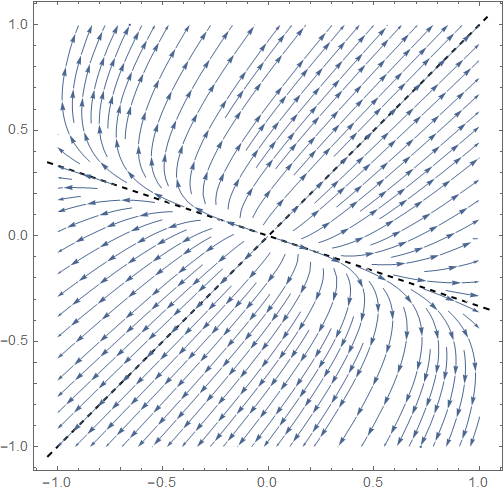
\includegraphics[width=0.8\linewidth]{964.png}}
\caption{Фазовый портрет Ф.: 964 (устойчивый узел)}
\label{964}
\end{figure}

\subsection{Ф.: 972*}
\begin{equation}
\begin{cases}
        \dot{x}=2x-y\\
        \dot{y}=x\\
    \end{cases}    
\end{equation}
Найдём собственные значения и собственные векторы матрицы $A=\begin{pmatrix}2 && -1 \\ 1 && 0 \end{pmatrix}$:\\
 $\lambda_1= 1,h_1 = \begin{pmatrix}1  \\  1 \end{pmatrix} $; $\lambda_2= 1,h_2 = h_1$. Нет базиса из собственных векторов. Поэтому ищем присоединённый: $h_{11} =\begin{pmatrix}1  \\  0 \end{pmatrix} $ Решением уравнения будет: $\vec x= C_1 \vec h_1 \exp{t}+C_2 ( \vec h_1 t + \vec h_{11})\exp{t}$. Положение равноевесия - неустойчивый вырожденный узел. 
 \begin{figure}[ht]
\center{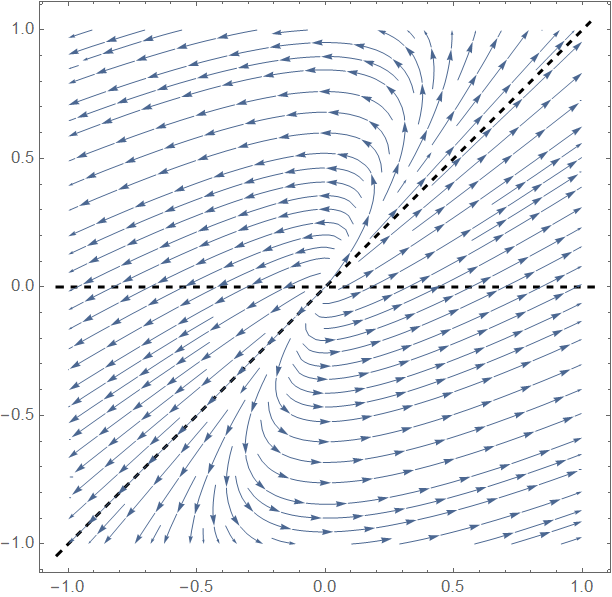
\includegraphics[width=0.8\linewidth]{972.png}}
\caption{Фазовый портрет Ф.: 972 (неустойчивый вырожденный узел) }
\label{972}
\end{figure}


\subsection{Ф.: 973}
Исследуем систему 
\begin{equation}
\begin{cases}
        \dot{x}=x+3y\\
        \dot{y}=-6x-5y\\
    \end{cases}    
\end{equation}
Найдём собственные значения и собственные векторы матрицы $A=\begin{pmatrix}1 && 3\\ -6 && -5 \end{pmatrix}$:\\
 $\lambda_1= -2+3i,h_1 = \begin{pmatrix} -1-i  \\  2 \end{pmatrix} $; $\lambda_2= -2-3i,h_2 = \begin{pmatrix} -1+i  \\  2 \end{pmatrix} $. Поскольку корни комплексные и $\Re{\lambda_{12}}<0$ , п.р. - устойчивый фокус. Построим фазовый портрет.
 \begin{figure}[ht]
\center{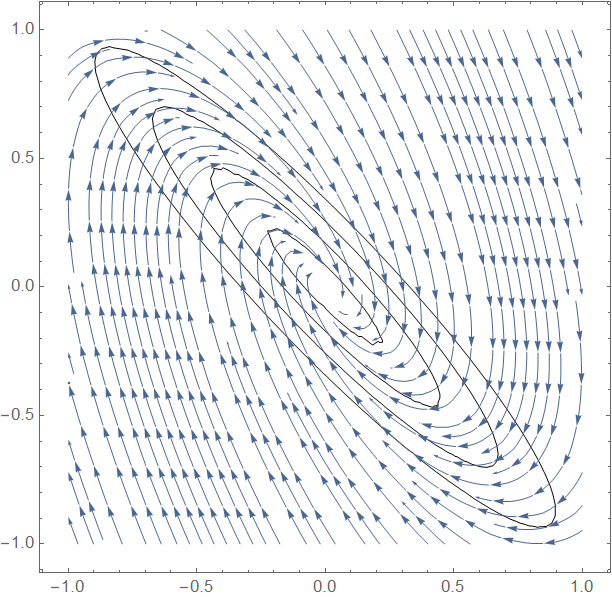
\includegraphics[width=0.8\linewidth]{973.png}}
\caption{Фазовый портрет Ф.: 973 (устойчивый фокус)}
\label{973}
\end{figure}
\textcolor[rgb]{1,1,1}{надо сказать, тут мешке сплохело и оно чутка корявое, надеюсь никто не почувствует слишком сильной эстетической боли}


\subsection{Ф.: 974}
Исследуем систему 
\begin{equation}
\begin{cases}
        \dot{x}=x\\
        \dot{y}=2x-y\\
    \end{cases}    
\end{equation}
Найдём собственные значения и собственные векторы матрицы $A=\begin{pmatrix}1 && 0 \\ 2 && -1 \end{pmatrix}$:\\
 $\lambda_1= -1,h_1 = \begin{pmatrix} 0  \\  1 \end{pmatrix} $; $\lambda_2= 1,h_2 = \begin{pmatrix} \pi  \\  \pi \end{pmatrix} $. Поскольку корни действительные и разных знаков, п.р. - седло. Построим фазовый портрет.
 \begin{figure}[ht]
\center{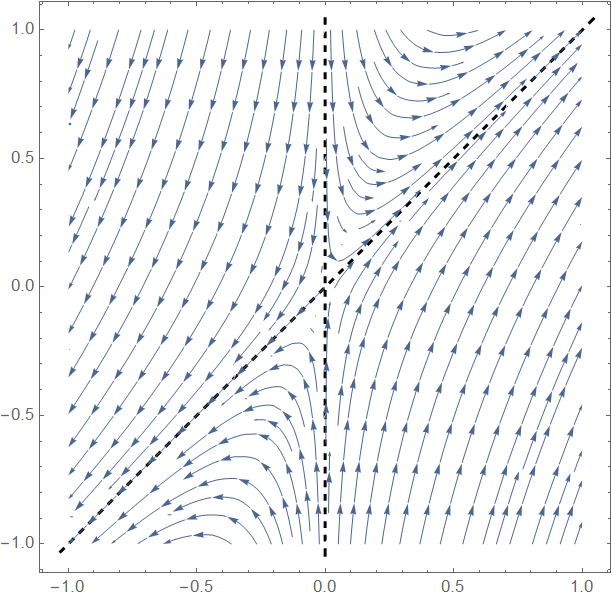
\includegraphics[width=0.8\linewidth]{974.png}}
\caption{Фазовый портрет Ф.: 974 (седло)}
\label{974}
\end{figure}\\

\subsection{Ф.: 975}
Исследуем систему 
\begin{equation}
\begin{cases}
        \dot{x}=-2x-5y\\
        \dot{y}=2x+2y\\
    \end{cases}    
\end{equation}
Найдём собственные значения и собственные векторы матрицы $A=\begin{pmatrix}-2 && -5 \\ 2 && 2 \end{pmatrix}$:\\
 $\lambda_1= i\sqrt6,h_1 = \begin{pmatrix} \frac{1}{2} \left(-2+i \sqrt{6}\right)  \\  1 \end{pmatrix} $; $\lambda_2= -i\sqrt6,h_2 = \begin{pmatrix} \frac{1}{2} \left(-2-i \sqrt{6}\right)  \\  1 \end{pmatrix} $. Поскольку корни комплексные и $\Re{\lambda_{12}}=0$ , п.р. - центр. Построим фазовый портрет.
 \begin{figure}[ht]
\center{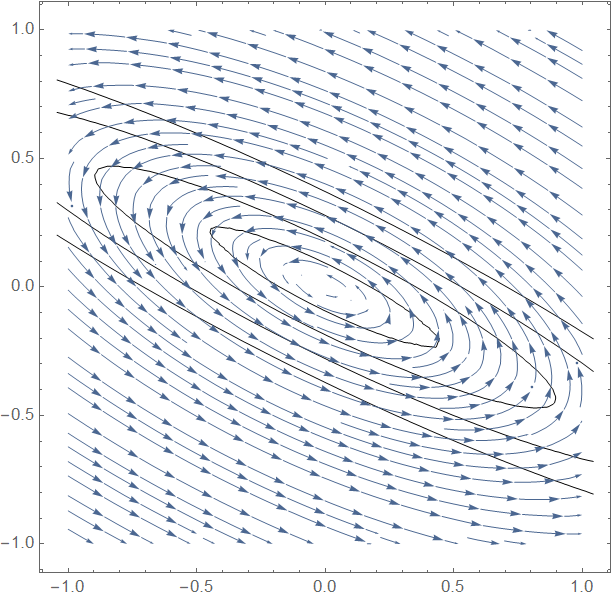
\includegraphics[width=0.8\linewidth]{975.png}}
\caption{Фазовый портрет Ф.: 975 (центр)}
\label{975}
\end{figure}\\

\subsection{Ф.: 978}
Исследуем систему 
\begin{equation}
\begin{cases}
        \dot{x}=-2x+y\\
        \dot{y}=-4x+2y\\
    \end{cases}    
\end{equation}
Найдём собственные значения и собственные векторы матрицы $A=\begin{pmatrix}-2 && 1 \\ -4 && 2 \end{pmatrix}$:\\
 $\lambda_1=0
 h_1 = \begin{pmatrix} 1  \\  2 \end{pmatrix} $; 
 $\lambda_2= 0,
 h_2 $ не существует, так что найдём присоединённый. \\
 $h_{11}= \begin{pmatrix} 0  \\  1 \end{pmatrix}$
 Я вообще без понятия, как называть п.р. с двумя нулевыми лямбдами. Но написать решение и нарисовать его можно. $\vec x = c_1 \vec h_1 + C_2 (\vec h_1 t + \vec h_{11})$
 \begin{figure}[ht]
\center{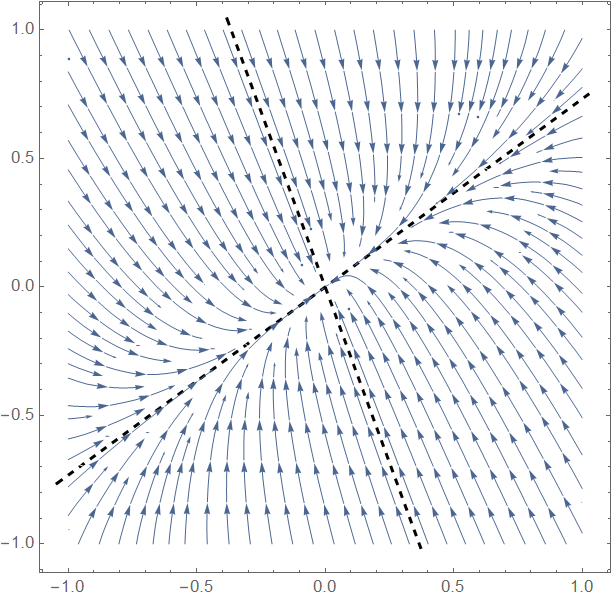
\includegraphics[width=0.8\linewidth]{978.png}}
\caption{Фазовый портрет Ф.: 978 (непойми что)}
\label{978}
\end{figure}\\

\subsection{С. \S13: 9}
Исследуем систему 
\begin{equation}
\begin{cases}
        \dot{x}=x^2+x+2y^2-2\\
        \dot{y}=x+y^2\\
    \end{cases}    
\end{equation}
Найдем точки равновесия, приравняв $\dot{x}=0; \dot{y}=0$ можем получить что точками равновесия будут: $p_1=(-1,1),p_2=(-1,-1)$\\
1)Лианеризуем (лианеризируем? лианеризовываем?) в $p_1$:\\
$x=u-1,y=v+1$:
\begin{equation}
\begin{cases}
        \dot{u}=-u+4v+o(u^2+v^2)\\
        \dot{v}=u+2v+o(v^2+u^2)\\
    \end{cases}    
\end{equation}
Найдём собственные значения и собственные векторы матрицы $A=\begin{pmatrix}-1 && 4 \\ 1 && 2 \end{pmatrix}$:\\
 $\lambda_1=3,
 h_1 = \begin{pmatrix} 1  \\  1 \end{pmatrix} $; 
 $\lambda_2= -2,
 h_2 = \begin{pmatrix} -4  \\  1 \end{pmatrix} $. 
 Поскольку корни действительные и разных знаков, п.р. - седло \ref{13.9.1}
 \begin{figure}[ht]
\center{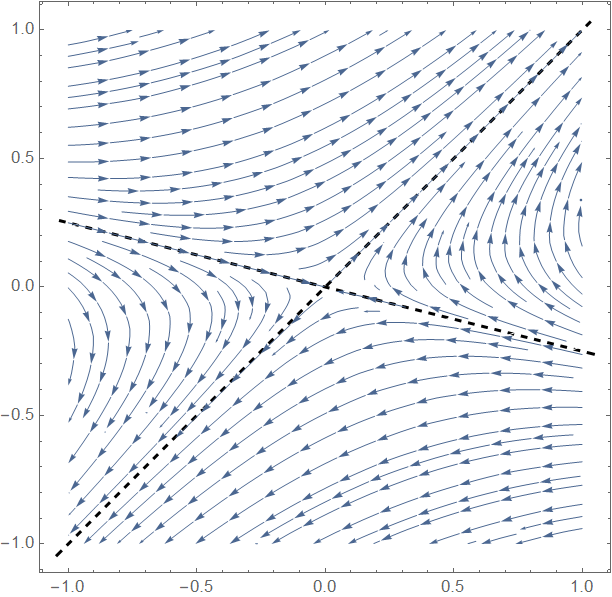
\includegraphics[width=0.8\linewidth]{13.9.1.png}}
\caption{Фазовый портрет С. \S13: 9 $(-1,1)$ (седло)}
\label{13.9.1}
\end{figure}\\
2)Лиан-что-то в $p_2$:\\
$x=u-1,y=v-1$:
\begin{equation}
\begin{cases}
        \dot{u}=-u-4v+o(u^2+v^2)\\
        \dot{v}=u-2v+o(v^2+u^2)\\
    \end{cases}    
\end{equation}
Найдём собственные значения и собственные векторы матрицы $A=\begin{pmatrix} -1 && -4 \\ 1 && -2 \end{pmatrix}$:\\
 $\lambda_1=\frac{1}{2} \left(-3+i \sqrt{15}\right),
 h_1 = \begin{pmatrix} \frac{1}{2} i \left(\sqrt{15}-i\right) \\  1 \end{pmatrix} $; 
 $\lambda_2= \frac{1}{2}\left(-3-i \sqrt{15}\right),
 h_2 = \begin{pmatrix} -\frac{1}{2} i \left(\sqrt{15}+i\right)  \\  1 \end{pmatrix} $. 
 Поскольку корни комплексные и $\Re \lambda_{12}<0$, п.р. - устойчивый фокус \ref{13.9.2}
 \begin{figure}[ht]
\center{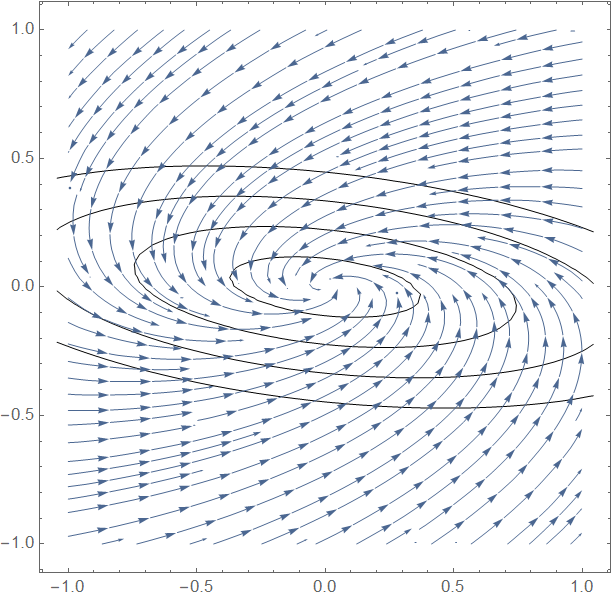
\includegraphics[width=0.8\linewidth]{13.9.2.png}}
\caption{Фазовый портрет С. \S13: 9 $(-1,-1)$ (устойчивый фокус)}
\label{13.9.2}
\end{figure}\\

А теперь построим весь фазовый портрет просто потому что можем \ref{13.9.3}.\\

\begin{figure}[ht]
\center{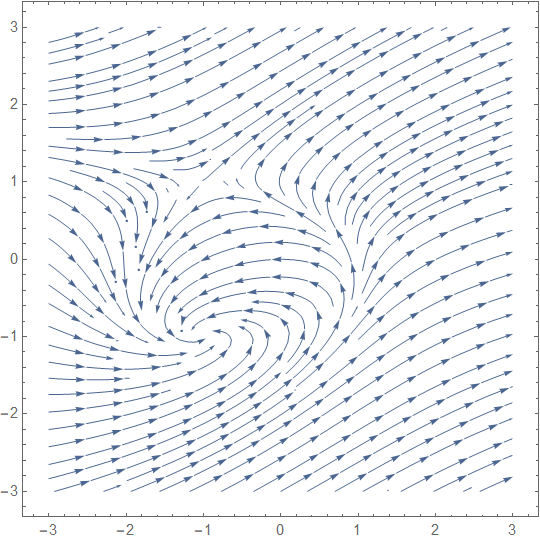
\includegraphics[width=0.8\linewidth]{13.9.3.png}}
\caption{Фазовый портрет С. \S13: 9  (просто красоты ради)}
\label{13.9.3}
\end{figure}

\subsection{С. \S13: 15}
Исследуем систему 
\begin{equation}
\begin{cases}
        \dot{x}=x^2-y\\
        \dot{y}=\ln{(3x^2-1)}-\ln{2}\\
    \end{cases}    
\end{equation}
Найдем точки равновесия, приравняв $\dot{x}=0; \dot{y}=0$ можем получить что точками равновесия будут: $p_1=(-1,1),p_2=(1,1)$\\

1)Лиан-что-то в $p_1$:\\
$x=u-1,y=v+1$:
\begin{equation}
\begin{cases}
        \dot{u}=-2u-v+o(u^2+v^2)\\
        \dot{v}=-3u+o(v^2)\\
    \end{cases}    
\end{equation}
Найдём собственные значения и собственные векторы матрицы $A=\begin{pmatrix} -2 && -1 \\ -3 && 0 \end{pmatrix}$:\\
 $\lambda_1=-3,
 h_1 = \begin{pmatrix} 1 \\  1 \end{pmatrix} $; 
 $\lambda_2= 1,
 h_2 = \begin{pmatrix} -1  \\  3 \end{pmatrix} $. 
 Поскольку корни действительные разных знаков, п.р. - седло \ref{13.15.1}
 \begin{figure}[ht]
\center{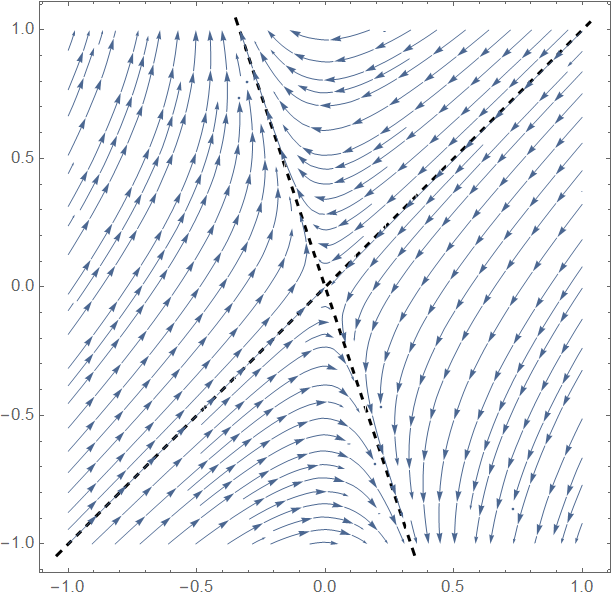
\includegraphics[width=0.8\linewidth]{13.15.1.png}}
\caption{Фазовый портрет С. \S13: 9 $(-1,1)$ (седло)}
\label{13.15.1}
\end{figure}\\

2)Лиан-что-то в $p_2$:\\
$x=u+1,y=v+1$:
\begin{equation}
\begin{cases}
        \dot{u}=2u-v+o(u^2+v^2)\\
        \dot{v}=3u+o(v^2+u^2)\\
    \end{cases}    
\end{equation}
Найдём собственные значения и собственные векторы матрицы $A=\begin{pmatrix}2 && -1 \\ 3 && 0 \end{pmatrix}$:\\
 $\lambda_1=1+i \sqrt{2},
 h_1 = \begin{pmatrix} \frac{1}{3} i \left(\sqrt{2}-i\right) \\  1 \end{pmatrix} $; 
 $\lambda_2= 1-i \sqrt{2}   ,
 h_2 = \begin{pmatrix} -\frac{1}{3} i \left(\sqrt{2}+i\right) \\  1 \end{pmatrix} $. 
 Поскольку корни комлексные и $\Re \lambda_{12}>0$, п.р. - неустойчивый фокус \ref{13.15.2}
 \begin{figure}[ht]
\center{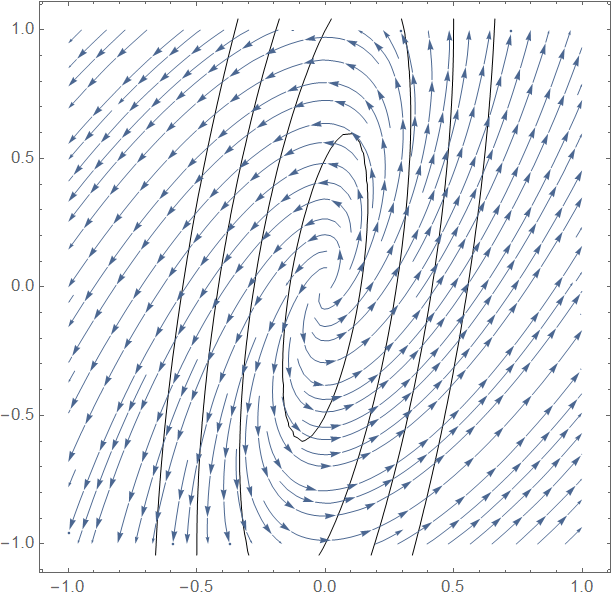
\includegraphics[width=0.8\linewidth]{13.15.2.png}}
\caption{Фазовый портрет С. \S13: 15 $(1,1)$ (неустойчивый фокус)}
\label{13.15.2}
\end{figure}\\


\subsection{С. \S13: 39}
Исследуем систему 
\begin{equation}
\begin{cases}
        \dot{x}=8+4y-2xy\\
        \dot{y}=x^2-4y^2\\
    \end{cases}    
\end{equation}
Найдем точки равновесия, приравняв $\dot{x}=0; \dot{y}=0$ можем получить что точками равновесия будут: $p_1=(-2,-1), p_2=(4,2)$\\

1)$p_1$:\\
$x=u-2,y=v-1$:
\begin{equation}
\begin{cases}
        \dot{u}=2u+8v+o(u^2+v^2)\\
        \dot{v}=-4u+8v+o(v^2)\\
    \end{cases}    
\end{equation}
Найдём собственные значения и собственные векторы матрицы $A=\begin{pmatrix} 2 && 8 \\ -4 && 8 \end{pmatrix}$:\\
 $\lambda_1=5+i \sqrt{23},
 h_1 = \begin{pmatrix} -\frac{1}{4} i \left(\sqrt{23}+3 i\right) \\  1 \end{pmatrix} $; 
 $\lambda_2= 5-i \sqrt{23},
 h_2 = \begin{pmatrix} \frac{1}{4} i \left(\sqrt{23}-3 i\right)  \\  3 \end{pmatrix} $. 
 Поскольку корни комплексные и $\Re \lambda_{12}>0$, п.р. - неустойчивый фокус \ref{13.39.1}
 \begin{figure}[ht]
\center{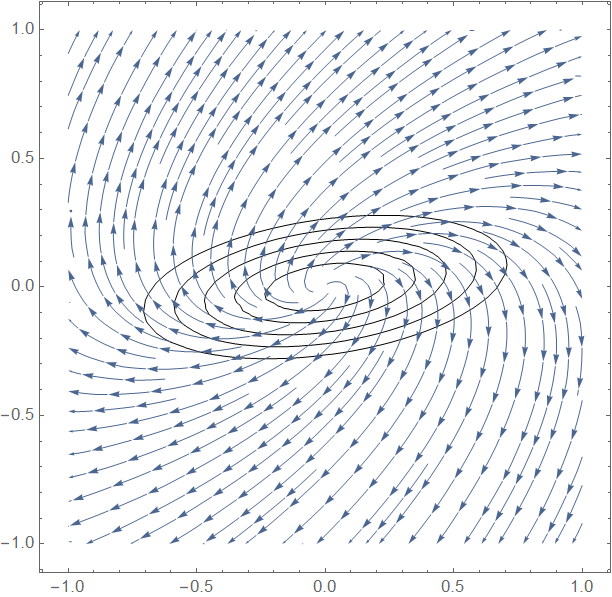
\includegraphics[width=0.8\linewidth]{13.39.1.png}}
\caption{Фазовый портрет С. \S13: 39 $(-2,-1)$ (неустойчивый фокус)}
\label{13.39.1}
\end{figure}\\  
2) $p_2$:\\
$x=u+4,y=v+2$:
\begin{equation}
\begin{cases}
        \dot{u}=-4u-4v+o(u^2+v^2)\\
        \dot{v}=8u-16v+o(v^2)\\
    \end{cases}    
\end{equation}
Найдём собственные значения и собственные векторы матрицы $A=\begin{pmatrix} -4 && -4 \\ 8 && -16 \end{pmatrix}$:\\
 $\lambda_1=-12,
 h_1 = \begin{pmatrix} 1 \\  2 \end{pmatrix} $; 
 $\lambda_2= -8,
 h_2 = \begin{pmatrix} 1 \\  1 \end{pmatrix} $. 
 Очевидно, п.р. - устойчивый узел \ref{13.39.2}
 \begin{figure}[ht]
\center{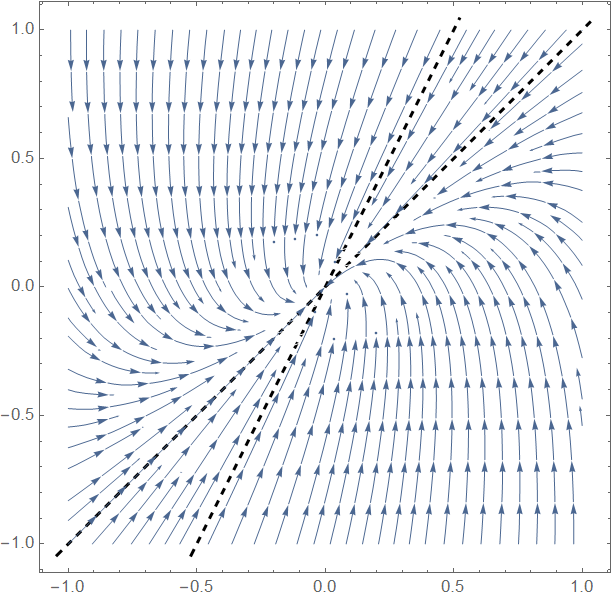
\includegraphics[width=0.8\linewidth]{13.39.2.png}}
\caption{Фазовый портрет С. \S13: 39 $(4,2)$ (устойчивый узел)}
\label{13.39.2}
\end{figure}\\  
Ну и картинка с 2 особыми точками, куда без неё: \ref{13.39.3}\\
 \begin{figure}[ht]
\center{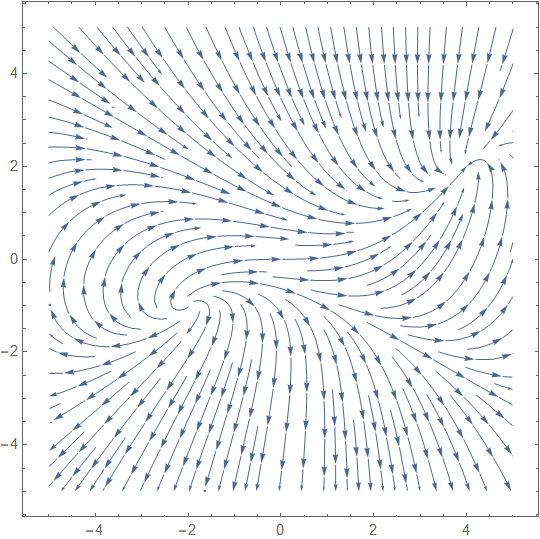
\includegraphics[width=0.8\linewidth]{13.39.3.png}}
\caption{Фазовый портрет С. \S13: 39}
\label{13.39.3}
\end{figure}\\

\subsection{С. \S13: 44}
Исследуем систему 
\begin{equation}
\begin{cases}
        \dot{x}=1-\exp{(x^2-y)}\\
        \dot{y}=\tanh{(2+x-x^2)}\\
    \end{cases}    
\end{equation}
Найдем точки равновесия, приравняв $\dot{x}=0; \dot{y}=0$ можем получить что точками равновесия будут: $p_1=(-1,1), p_2=(2,4)$\\

1)$p_1$:\\
$x=u-1,y=v+1$:
\begin{equation}
\begin{cases}
        \dot{u}=2u+v+o(u^2+v^2)\\
        \dot{v}=3u+0v+o(v^2)\\
    \end{cases}    
\end{equation}
Найдём собственные значения и собственные векторы матрицы $A=\begin{pmatrix} 2 && 1 \\ 3 && 0 \end{pmatrix}$:\\
 $\lambda_1=3,
 h_1 = \begin{pmatrix} 1 \\  1 \end{pmatrix} $; 
 $\lambda_2= -1,
 h_2 = \begin{pmatrix} -1 \\  3 \end{pmatrix} $. 
 Очевидно, п.р. - седло \ref{13.44.1}
 \begin{figure}[ht]
\center{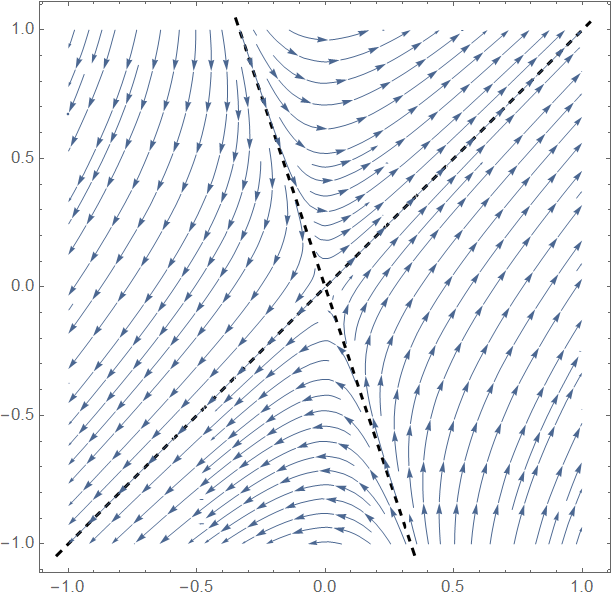
\includegraphics[width=0.8\linewidth]{13.44.1.png}}
\caption{Фазовый портрет С. \S13: 44 $(-1,1)$ (седло)}
\label{13.44.1}
\end{figure}\\  
2) $p_2$:\\
$x=u+2,y=v+4$:
\begin{equation}
\begin{cases}
        \dot{u}=-4u+v+o(u^2+v^2)\\
        \dot{v}=-3u+o(v^2)\\
    \end{cases}    
\end{equation}
Найдём собственные значения и собственные векторы матрицы $A=\begin{pmatrix} -4 && 1 \\ -3 && 0 \end{pmatrix}$:\\
 $\lambda_1=-3,
 h_1 = \begin{pmatrix} 1 \\  1 \end{pmatrix} $; 
 $\lambda_2= -1,
 h_2 = \begin{pmatrix} 1 \\  3 \end{pmatrix} $. 
 Очевидно, п.р. - устойчивый узел \ref{13.44.2}
 \begin{figure}[ht]
\center{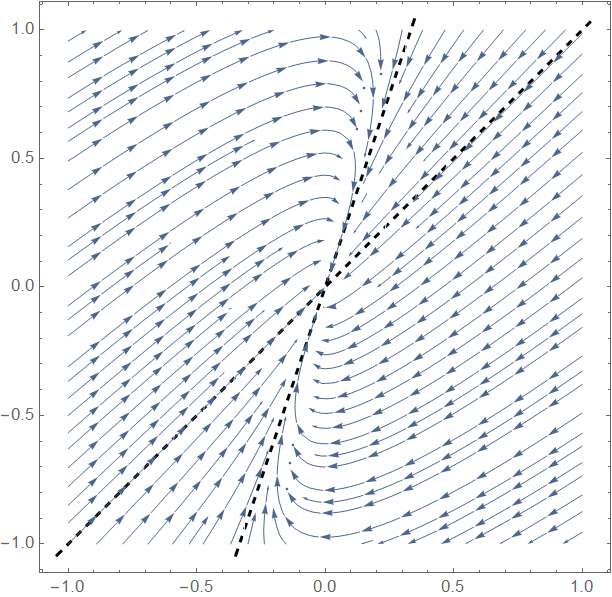
\includegraphics[width=0.8\linewidth]{13.44.2.png}}
\caption{Фазовый портрет С. \S13: 44 $(2,4)$ (устойчивый узел)}
\label{13.44.2}
\end{figure}\\  
Ну и картинка с 2 особыми точками, куда без неё\ref{13.44.3}:\\
 \begin{figure}[ht]
\center{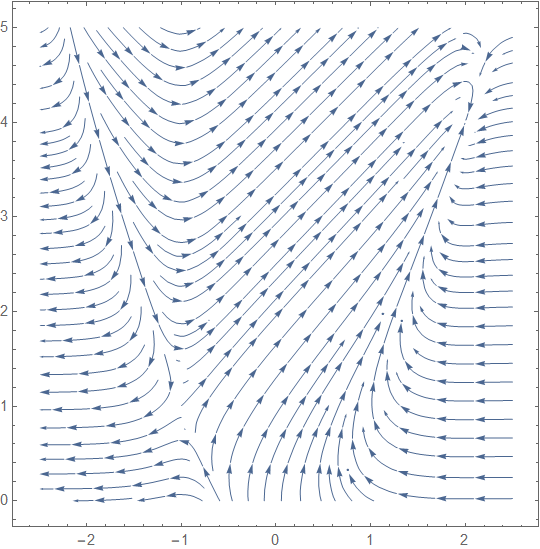
\includegraphics[width=0.8\linewidth]{13.44.3.png}}
\caption{Фазовый портрет С. \S13: 44}
\label{13.44.3}
\end{figure}\\

\subsection{С. \S13: 45}
Исследуем систему 
\begin{equation}
\begin{cases}
        \dot{x}=\sqrt{1+2x-5y}-1\\
        \dot{y}=\arctg{(x/2+3/5x^2-2y)}\\
    \end{cases}    
\end{equation}
Найдем точки равновесия, приравняв $\dot{x}=0; \dot{y}=0$ можем получить что точками равновесия будут: $p_1=(0,0), p_2=(1/2,1/5)$\\

1)$p_1$:\\
$x=u,y=v$:
\begin{equation}
\begin{cases}
        \dot{u}=u-5/2v+o(u^2+v^2)\\
        \dot{v}=1/2u-2v+o(v^2)\\
    \end{cases}    
\end{equation}
Найдём собственные значения и собственные векторы матрицы $A=\begin{pmatrix} 1 && -5/2 \\ 1/2 && -2 \end{pmatrix}$:\\
 $\lambda_1=-3/2,
 h_1 = \begin{pmatrix} 1 \\  1 \end{pmatrix} $; 
 $\lambda_2= 1/2,
 h_2 = \begin{pmatrix} 5 \\  1 \end{pmatrix} $. 
 Очевидно, п.р. - седло \ref{13.45.1}
 \begin{figure}[ht]
\center{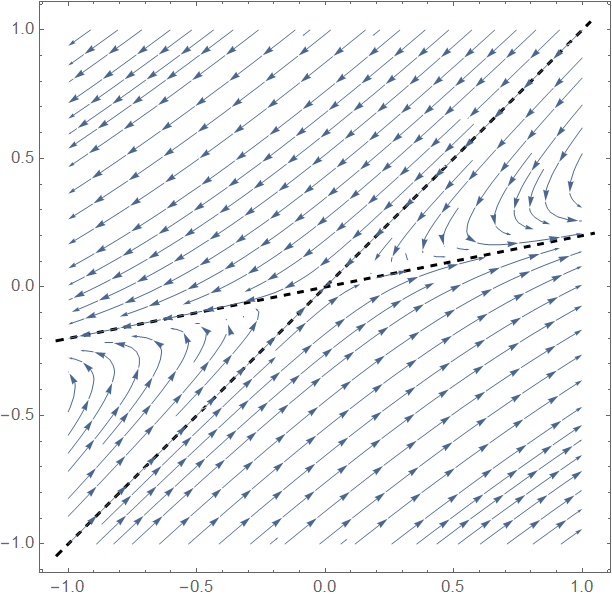
\includegraphics[width=0.8\linewidth]{13.45.1.png}}
\caption{Фазовый портрет С. \S13: 45 $(0,0)$ (седло)}
\label{13.45.1}
\end{figure}\\ 

2) $p_2$:\\
$x=u+1/2,y=v+1/5$:
\begin{equation}
\begin{cases}
        \dot{u}=u-5/2v+o(u^2+v^2)\\
        \dot{v}=11/10u-2v+o(v^2)\\
    \end{cases}    
\end{equation}
КТО ПРИДУМАЛ ЭТИ ЧИСЛА?!?!?!? Простите, крик боли утсавшего человека, который не поужинает, пока не закончит дифуры.\\
Найдём собственные значения и собственные векторы матрицы $A=\begin{pmatrix} 1 && -5/2 \\ 11/10 && -2 \end{pmatrix}$:\\
 $\lambda_1=\frac{1}{2} \left(-1+i \sqrt{2}\right),
 h_1 = \begin{pmatrix}\frac{5}{11} i \left(\sqrt{2}-3 i\right) \\  1 \end{pmatrix} $; 
 $\lambda_2= \frac{1}{2} \left(-1-i \sqrt{2}\right),
 h_2 = \begin{pmatrix} \frac{1}{11} (-5) i \left(\sqrt{2}+3 i\right) \\  1 \end{pmatrix} $. 
 Очевидно, п.р. - устойчивый фокус \ref{13.45.2}
 \begin{figure}[ht]
\center{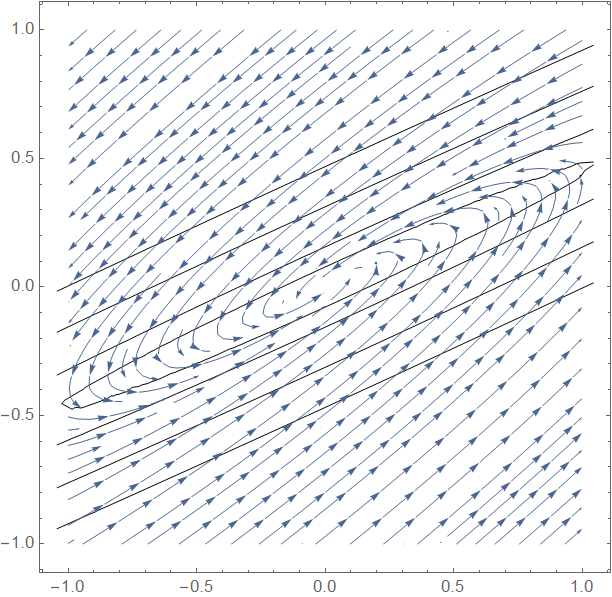
\includegraphics[width=0.8\linewidth]{13.45.2.png}}
\caption{Фазовый портрет С. \S13: 45 $(1/2,1/5)$ (устойчивый фокус)}
\label{13.45.2}
\end{figure}\\  
Ну и картинка с 2 особыми точками, куда без неё (только там беды с корнем на некоторой области и она не такая красивая): \ref{13.45.3}\\
 \begin{figure}[ht]
\center{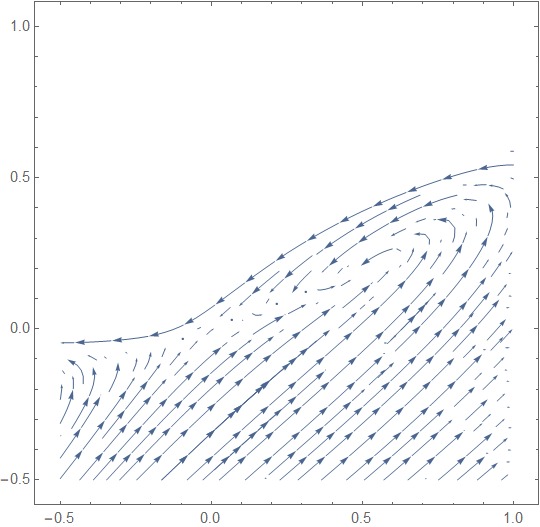
\includegraphics[width=0.8\linewidth]{13.45.3.png}}
\caption{Фазовый портрет С. \S13: 45}
\label{13.45.3}
\end{figure}\\
\end{document}
